% Ad Hoc Networks (Elsevier) — Submission Draft
% Adapted from IOTJ-Aug.tex
% Target: Ad Hoc Networks (ISSN 1570-8705, IF ~4.8)
% Abbrev: Ad Hoc Netw.
%
\documentclass[preprint,12pt]{elsarticle}

\usepackage[T1]{fontenc}
\usepackage[utf8]{inputenc}
\usepackage{enumitem}
\usepackage{amsmath,amssymb,amsthm}
\usepackage{booktabs}
\usepackage{array}
\usepackage{multirow}
\usepackage{graphicx}
\usepackage{float}
\usepackage{xcolor}
\usepackage{url}
\usepackage{listings}
\usepackage{algorithm2e}
\usepackage{tikz}
\usetikzlibrary{shapes.geometric,arrows.meta,positioning,fit,calc,backgrounds}
\usepackage[hidelinks]{hyperref}
\emergencystretch=2em

% Theorem environments for formal definitions
\newtheorem{definition}{Definition}
\newtheorem{property}{Security Property}
\newtheorem{remark}{Remark}

\lstset{
  basicstyle=\ttfamily\footnotesize,
  breaklines=true,
  frame=single,
  xleftmargin=2em,
}

% ------------------------------------------------------------------
\begin{document}

\begin{frontmatter}

\title{Securing LoRa Mesh Ad~Hoc Networks: Formal Vulnerability
       Analysis and Lightweight Authenticated Routing}

\author[inst1]{[Author Names]}
\address[inst1]{[Institution, Country]}
\ead{[email]}

\begin{abstract}
LoRaMesher, a widely used open-source distance-vector mesh routing
stack for ESP32-class LoRa nodes, carries no cryptographic
authentication on its control plane, exposing it to route injection
by any attacker with a commodity \$20 LoRa transceiver.

Successful route injection is shown to produce a \emph{silent
traffic black hole}, not an adversarial relay.
The root cause is a cross-layer semantic mismatch: the deployed
firmware encodes next-hop forwarding state in the destination
field rather than the final-gateway identity assumed by symbolic
and packet-level analyses.
This mismatch is invisible to both Tamarin formal models and ns-3
packet-level simulation; it becomes observable only through
physical hardware serial-log inspection.

This paper addresses the gap through a three-tier methodology:
Tamarin machine-checked proofs confirming four attack lemmas on
the unpatched protocol, ns-3 simulation across 135 scenarios and
up to 49 nodes, and validation on six physical EoRa-PI boards.
A lightweight patch is proposed—HMAC-SHA256 per-message
authentication combined with a per-destination MetricVersion
counter—requiring no PKI infrastructure.
No attack-induced PDR degradation is observed under any tested
condition, and all artifacts are publicly released.
\end{abstract}

\begin{keyword}
LoRa \sep ad hoc mesh routing \sep distance-vector routing security
\sep silent traffic black hole \sep cross-layer semantic mismatch
\sep routing forwarding semantics \sep formal verification
\sep Tamarin Prover \sep HMAC authentication
\sep route injection \sep replay attack \sep ESP32
\end{keyword}

\end{frontmatter}

% ==================================================================
\section{Introduction}
\label{sec:intro}
% ==================================================================

LoRa-based ad~hoc mesh networks have achieved remarkable
deployment scale.
Individual installations now span hundreds of sensor nodes across
farmland, mountain ranges, and urban districts.
Multi-hop distance-vector (DV) routing is used to relay data
where fixed infrastructure is absent or cost-prohibitive~\cite{ieee2025-lora-hierarchy-routing}.
LoRaMesher~\cite{sole2022-loramesher,sole2024-loramesher-dv,sole2026-loramesher-swx,repetto2022-lorawan-demo}
is at the core of many such deployments:
an open-source mesh routing stack for ESP32-class nodes
(240~MHz, 512~KB RAM) providing route discovery, neighbor
management, and session rekeying without fixed infrastructure.
Despite its growing adoption, \emph{the security of
LoRaMesher's control-plane messages has not been formally
analyzed}.
To our knowledge, no prior published work has produced
machine-checked vulnerability proofs for any LoRa mesh routing
protocol, proposed a formally verified patch, or validated the
result across multi-topology simulation and physical hardware.

\subsection{The Deployment Security Problem}

Ad hoc mesh deployments operate in adversarial physical environments:
sensor nodes are unattended in open fields, accessible to any
actor with a \$20 LoRa transceiver. Despite this exposure,
LoRaMesher's control plane—responsible for Hello broadcasts,
route discovery, and 30-second session rekeying—carries no
cryptographic authentication. This design gap creates two practical
attack vectors available to any adversary with commodity hardware:

\begin{enumerate}
  \item \textbf{Route Injection}: An attacker transmits a forged
    Hello claiming a minimum-metric path to the gateway.
    Without authentication, all mesh nodes converge their routing
    tables to the attacker within one DV cycle ($\approx$30~s).
    Because LoRaMesher's firmware encodes the next-hop address in
    the destination field, all subsequent data packets carry
    \texttt{dst=attacker}—and the gateway silently receives
    none of them, creating a complete traffic black hole with
    no observable anomaly at the legitimate receiver.

  \item \textbf{Session Replay}: An attacker captures a legitimate
    RekeyNotice and replays it after the mesh advances to a new
    session epoch. Nodes that accept the stale epoch can be made
    to decrypt traffic with a compromised old key.
\end{enumerate}

Both attacks share a common structural root cause.
LoRaMesher's control plane treats received messages as equally
authoritative without verifying sender identity or message
freshness.
This design—inherited from classical DV routing built for
trusted wired networks—creates an \emph{adversarial state
injection surface}: the routing state of the entire mesh can be
permanently corrupted by a single well-timed control message
from any node within radio range.
The two attack classes are therefore two manifestations of the
same missing property: authenticated state transitions in a
broadcast medium.

Neither attack requires node compromise or cryptographic break—only
a commodity LoRa radio.
Both are reproduced in ns-3 with 100\% success rate on linear
topologies.

\subsection{Why Existing Solutions Do Not Apply}

LoRaWAN security~\cite{ieee2025-lorawan-key-vulnerability,ieee2025-lorawan-key-verification,mohamed2022-lorawan-gateways,butun2019-lorawan-security-risk}
targets the star-topology WAN layer managed by network servers;
no mechanism for mesh control-plane authentication is provided.
Standard mesh security protocols—802.15.4 CCM*, AODV-SEC~\cite{hu2002-sead},
and ARIADNE~\cite{hu2002-ariadne}—assume PKI infrastructure or
TESLA-based one-way chains requiring clock synchronisation.
Both prerequisites are infeasible under LoRa's duty-cycle and
sleep-cycle constraints.
Lightweight asymmetric alternatives such as
TinyECC~\cite{liu2008-tinyecc} require $>$500~ms per operation
on ESP32—prohibitive at a 10-second Hello interval.
As documented in existing surveys~\cite{hessel2022-lorawan-survey,butun2019-lorawan-security-risk},
deployed LPWAN protocols frequently lack formal security
analysis, leaving them exposed to well-known attack classes.

\textbf{The gap.} Existing work has addressed LoRaWAN WAN-layer
security and generic mesh routing security separately, but none has
jointly (i)~formally characterized vulnerabilities in the LoRa mesh
routing control plane with machine-checked proofs, (ii)~proposed
and formally verified a corrective patch satisfying all security
goals, and (iii)~validated the outcome across multi-topology
simulation and physical hardware experiments. This paper closes
that gap.

\subsection{Key Observation}
\label{sec:key-observation}

Physical hardware validation reveals a finding that formal and
simulation analysis cannot capture: route injection creates a
\emph{silent traffic black hole}, not an adversarial relay.
The deployed firmware encodes the next-hop address in the
\texttt{dst} field; the gateway silently drops every arriving
packet because $\texttt{dst} \neq \texttt{0xBB}$, producing
zero observable anomaly at the legitimate receiver.
The mechanism and its implications for intrusion detection design
are developed in full in Section~\ref{sec:cross-layer}; the key
consequence for deployment is that an IDS monitoring the gateway
observes only silence.

\subsection{Contributions}

This paper makes three contributions:

\begin{enumerate}

  \item \textbf{Cross-Layer Routing Semantics Finding.}
    Route injection in LoRaMesher is identified to create a
    \emph{silent traffic black hole}—not an adversarial relay—because
    the deployed firmware encodes next-hop forwarding state in the
    \texttt{dst} field rather than the final gateway identity assumed
    by protocol-layer analyses.
    This cross-layer semantic mismatch:
    (i)~is invisible to both Tamarin symbolic analysis and
    ns-3 packet-level simulation;
    (ii)~explains the topology-dependent PDR gradient
    (0\% on linear; 22.6\% degradation on tree and grid) as a
    structural consequence of next-hop entry count per path;
    (iii)~becomes visible only through physical hardware serial-log
    inspection; and
    (iv)~changes the threat model from adversarial relay to confirmed
    black hole, with direct implications for intrusion detection
    design—gateway-centric IDS observes only silence
    (Section~\ref{sec:cross-layer}).

  \item \textbf{Three-Tier Verification Methodology That Makes the
    Finding Visible.}
    We develop a progressive verification pipeline in which each tier
    reveals a distinct aspect of the vulnerability:
    (a)~\emph{Tamarin formal analysis} identifies the control-plane
    vulnerability class via machine-checked counterexample traces
    (four of five baseline lemmas falsified) and verifies a
    corrective lightweight patch—HMAC-SHA256 per-message
    authentication and a NVS-persistent MetricVersion counter—
    satisfying all security goals with no PKI dependency;
    (b)~\emph{ns-3 multi-topology simulation} quantifies PDR impact
    across three topologies and scales up to 49~nodes;
    (c)~\emph{physical hardware validation} on six EoRa-PI boards
    is the only tier capable of revealing the dst-as-next-hop
    encoding—and thus the correct attack semantics
    (Sections~\ref{sec:formal}–\ref{sec:eval}).

  \item \textbf{Open Reproducible Artifact Suite.}
    All Tamarin models, ns-3 simulation code, patched firmware,
    and hardware serial logs are publicly released
    (Appendix~\ref{app:artifact}).

\end{enumerate}

\subsection{Methodology Overview}
\label{sec:methodology}

Our study follows a four-phase, mutually corroborating methodology:

\begin{enumerate}[label=\textbf{Phase \arabic*.}]
  \item \textbf{Formal Disclosure} (Section~\ref{sec:formal}):
    A Tamarin Prover model of LoRaMesher's control plane is
    constructed and machine-checked attack traces are derived.
    This bounds the vulnerability precisely: the exact state
    transitions enabling each attack are identified without reliance
    on testing intuition.

  \item \textbf{Verified Patch} (Section~\ref{sec:patch}):
    The Tamarin model is extended with proposed patch rules and all
    security lemmas are re-verified. The patch is accepted only when
    Tamarin proves all 8 goals, guaranteeing it eliminates the
    formally identified root causes—not just the observed symptoms.

  \item \textbf{Multi-Topology Simulation} (Section~\ref{sec:eval}):
    The protocol, both attacks, and three security modes are
    implemented in ns-3.40 with a C++17 Dolev-Yao attacker,
    translating Tamarin's symbolic guarantees into packet-level
    PDR measurements across linear, tree, and grid topologies.

  \item \textbf{Physical Hardware Validation}
    (Section~\ref{sec:hardware-validation}):
    We reproduce the attack and patch on Ebyte EoRa-PI boards
    (ESP32-S3 + SX1262). Hardware serial logs reveal the
    \texttt{dst}-as-next-hop encoding that neither formal model
    nor simulator captures—establishing the correct attack
    semantics (silent black hole, not adversarial relay).
\end{enumerate}

The phases are not redundant: formal proofs bound the
vulnerability class precisely; simulation quantifies
deployment-scale PDR impact; hardware reveals forwarding
semantics that neither formal nor simulation models capture.

\begin{figure*}[!t]
\centering
\definecolor{attackred}{RGB}{163,45,45}
\definecolor{attackbg}{RGB}{252,235,235}
\definecolor{defensegreen}{RGB}{15,110,86}
\definecolor{defensebg}{RGB}{225,245,238}
\definecolor{nodegray}{RGB}{136,135,128}
\definecolor{nodebg}{RGB}{241,239,232}
\definecolor{infogray}{RGB}{95,94,90}

\resizebox{\textwidth}{!}{%
\begin{tikzpicture}[
    font=\sffamily\footnotesize,
    node distance=0.6cm,
    meshnode/.style={
        circle, draw=nodegray, fill=nodebg,
        line width=0.4pt, minimum size=0.88cm,
        inner sep=1pt, font=\sffamily\scriptsize
    },
    ghostnode/.style={
        circle, draw=gray!40, fill=gray!10,
        line width=0.4pt, minimum size=0.88cm,
        inner sep=1pt, font=\sffamily\scriptsize, text=gray!60
    },
    attacker/.style={
        rectangle, draw=attackred, fill=attackbg,
        line width=0.5pt, rounded corners=2pt,
        minimum width=1.45cm, minimum height=0.88cm,
        inner sep=2pt, align=center,
        font=\sffamily\scriptsize
    },
    semanticbox/.style={
        rectangle, line width=0.55pt, rounded corners=2pt,
        minimum width=5.25cm, minimum height=0.64cm,
        inner sep=3pt, align=center,
        font=\sffamily\small\bfseries
    },
    resultbox/.style={
        rectangle, line width=0.65pt, rounded corners=3pt,
        minimum width=5.8cm, minimum height=0.82cm,
        inner sep=4pt, align=center,
        font=\sffamily\small\bfseries
    },
    smallnote/.style={
        rectangle, draw=nodegray, fill=nodebg,
        line width=0.35pt, rounded corners=2pt,
        minimum width=4.8cm, minimum height=0.46cm,
        inner sep=2pt, align=center,
        font=\sffamily\tiny, text=infogray
    },
    dropbox/.style={
        rectangle, draw=attackred, fill=attackbg,
        line width=0.7pt, rounded corners=2pt,
        minimum width=1.2cm, minimum height=0.5cm,
        inner sep=2pt, align=center,
        font=\sffamily\scriptsize\bfseries, text=attackred
    },
    relaybox/.style={
        rectangle, draw=attackred, fill=attackbg,
        line width=0.7pt, rounded corners=2pt,
        minimum width=1.2cm, minimum height=0.5cm,
        inner sep=2pt, align=center,
        font=\sffamily\scriptsize\bfseries, text=attackred
    },
    stepmark/.style={
        circle, draw=nodegray, fill=white,
        line width=0.35pt, minimum size=0.32cm,
        inner sep=0pt, font=\sffamily\tiny\bfseries,
        text=infogray
    },
    panel title/.style={font=\sffamily\small\bfseries},
    panel subtitle/.style={font=\sffamily\scriptsize, text=infogray},
    packetarrow/.style={
        -{Stealth[length=1.8mm, width=1.8mm]},
        line width=0.75pt, draw=attackred
    },
    relayarrow/.style={
        -{Stealth[length=1.8mm, width=1.8mm]},
        line width=0.75pt, draw=attackred, dashed,
        dash pattern=on 2pt off 1.5pt
    },
    silentarrow/.style={
        -{Stealth[length=1.5mm, width=1.5mm]},
        line width=0.45pt, draw=gray!45, dashed,
        dash pattern=on 1.5pt off 1.5pt
    },
    arrowlabel/.style={
        font=\sffamily\scriptsize, text=attackred,
        fill=white, inner sep=1pt
    },
    graylabel/.style={
        font=\sffamily\scriptsize, text=infogray,
        fill=white, inner sep=1pt
    }
]

% ============================================================
% LEFT PANEL: Protocol-layer model prediction
% ============================================================
\node[panel title] (ltitle) at (-4.35, 4.25)
    {Protocol Abstraction};
\node[panel subtitle, below=0.03cm of ltitle]
    {Tamarin symbolic model + ns-3 packet model};

\node[semanticbox, draw=attackred, fill=attackbg, text=attackred]
    at (-4.35, 3.25) {\texttt{dst} = final destination};

\node[meshnode] (LA) at (-6.8, 2.15) {A};
\node[attacker] (LE) at (-4.35, 2.15) {Attacker};
\node[meshnode] (LG) at (-1.9, 2.15) {GW};

\draw[packetarrow] (LA) -- (LE);
\draw[relayarrow] (LE) -- (LG)
    node[arrowlabel, above=5pt, midway] {redirected traffic};

\node[stepmark] at (-5.65, 2.45) {1};
\node[relaybox] at (-4.35, 1.2) {RELAY};
\draw[packetarrow] (LE) -- (-4.35,1.47);
\node[stepmark] at (-3.15, 2.72) {2};

\node[resultbox, draw=attackred, fill=attackbg, text=attackred]
    at (-4.35, 0.30) {Adversarial relay predicted};

\node[font=\sffamily\scriptsize, text=infogray, align=center]
    at (-4.35, -0.45) {Gateway monitor expects anomalous traffic};

\node[smallnote] at (-4.35, -1.12)
    {Model artifact: packets are routed to the attacker's node address};

% ============================================================
% DIVIDER
% ============================================================
\draw[draw=nodegray, line width=0.35pt, dashed,
      dash pattern=on 1.5pt off 1.5pt]
    (0, 4.55) -- (0, -1.45);

% ============================================================
% RIGHT PANEL: Firmware reality (hardware validation)
% ============================================================
\node[panel title] (rtitle) at (4.35, 4.25)
    {Firmware Reality};
\node[panel subtitle, below=0.03cm of rtitle]
    {Hardware-level validation};

\node[semanticbox, draw=defensegreen, fill=defensebg, text=defensegreen]
    at (4.35, 3.25) {\texttt{dst} = next hop};

\node[meshnode] (RA) at (1.85, 2.15) {A};
\node[meshnode] (RB) at (4.35, 2.15) {B};
\node[ghostnode] (RG) at (6.85, 2.15) {GW};

\draw[packetarrow] (RA) -- (RB);
\node[stepmark] at (3.05, 2.45) {1};
\node[dropbox] (DROP) at (4.35, 1.2) {DROP};
\draw[packetarrow] (RB) -- (DROP)
    node[arrowlabel, right, midway] {not for me};
\draw[silentarrow] (RB) -- (RG)
    node[graylabel, above=5pt, midway] {no traffic reaches GW};
\node[stepmark] at (3.95, 1.66) {2};
\node[stepmark] at (5.65, 2.72) {3};

\node[font=\sffamily\scriptsize, text=gray!70, align=center]
    at (6.85, 1.22) {IDS sees\\silence};

\node[resultbox, draw=defensegreen, fill=defensebg, text=defensegreen]
    at (4.35, 0.22) {Silent black hole discovered};

\node[font=\sffamily\scriptsize, text=defensegreen, align=center]
    at (4.35, -0.52) {Gateway-centric IDS observes only silence};

\node[smallnote] at (4.35, -1.08)
    {Topology determines black-hole spread};

\end{tikzpicture}%
}

\caption{Protocol-layer abstraction predicts traffic interception, but
deployed firmware creates a silent black hole.
Protocol-layer analyses interpret \texttt{dst} as the final destination,
so route injection appears to redirect traffic through an adversarial
relay. Hardware-level validation shows that LoRaMesher instead writes
the next-hop address into \texttt{dst}: the relay treats the packet as
not addressed to itself, drops it, and the gateway-side IDS observes
only silence.}
\label{fig:hero}
\end{figure*}

% ==================================================================
\section{Ad Hoc Network Deployment Context and Threat Model}
\label{sec:threat}
% ==================================================================

\subsection{Target Deployment Scenarios}

We target three representative LoRa mesh deployment classes:

\begin{itemize}
  \item \textbf{Precision Agriculture}: 20–100 soil sensors deployed
    across a 50~ha field, relaying pH, moisture, and temperature
    data through a 6-hop linear mesh to a field gateway.
    Attack impact: falsified soil data causes mis-irrigation.

  \item \textbf{Disaster-Response Networks}: Ad-hoc mesh deployed
    by first responders across a disaster zone. Gateway-reachability
    is critical for coordination. Attack impact: route hijacking
    isolates field teams.

  \item \textbf{Smart City Infrastructure}: 3×3 grid of air-quality
    nodes in urban blocks. Nodes are physically accessible.
    Attack impact: replay attacks create false pollution readings.
\end{itemize}

\subsection{ESP32 Resource Constraints}

Our patch must operate within ESP32-S3 constraints:

\begin{table}[t]
  \centering
  \caption{ESP32-S3 Resource Budget for LoRaMesher Security Patch}
  \label{tab:esp32}
  \resizebox{0.98\textwidth}{!}{%
  \begin{tabular}{lcc}
    \toprule
    \textbf{Resource} & \textbf{Available} & \textbf{Patch Overhead} \\
    \midrule
    Flash              & 8~MB             & 2.1~KB (+0.03\%) \\
    SRAM               & 512~KB           & 2~B/route entry (\texttt{uint16} MV, 7.6-day exhaust at 10\,s interval) \\
    CPU (HMAC-SHA256)  & 240~MHz          & 0.098~ms/message \\
    LoRa link latency  & 100–250~ms       & CPU overhead $<$0.1\% \\
    LoRa airtime (Hello) & 124~ms (SF9)  & 206~ms patched (+66\%) \\
    Duty cycle (Hello) & 1.24\%/10~s    & 2.06\%/10~s (+0.82 pp) \\
    Battery (baseline) & 2500~mAh         & $<$0.5\% additional draw \\
    \bottomrule
  \end{tabular}
  }
\end{table}

The HMAC computation time (0.098~ms on ESP32-S3, measured with
mbedTLS~2.28 on production hardware, 10{,}000 iterations) is three
orders of magnitude smaller than LoRa's minimum air-time and is
therefore computationally negligible.

\textbf{LoRa airtime and duty-cycle impact.}
The patch appends a 16-byte HMAC-SHA256 tag (truncated to 128~bits)
to each control message, consistent with the implementation
in Section~\ref{sec:patch} and the Tamarin model in
Section~\ref{sec:formal}. Using the Semtech LoRa ToA formula at
SF9 / BW=125~kHz / CR=4/5 / explicit header / CRC:
a Hello message grows from 6~bytes (baseline) to 22~bytes (patched),
increasing time-on-air from $\approx$124~ms to $\approx$206~ms
(+66\%). The per-node duty-cycle increase for Hello traffic is
$(206-124)/10{,}000 = 0.82$~percentage points. For a minimal sensor data packet
(13~bytes $\to$ 29~bytes), the airtime increase is $\approx$37\%;
the 64-byte simulation payload (64~bytes $\to$ 80~bytes) increases
airtime by $\approx$16\%.
In the AS923 band (used in this study), the 1\% per-channel
duty-cycle ceiling applies; the additional $\approx$0.82~pp overhead
from Hellos remains within this ceiling for nodes sending one Hello
per 10~s period. Operators with tighter duty-cycle budgets may
reduce HMAC to 8~bytes (64-bit tag), halving the airtime overhead
at the cost of reduced security margin.

\subsection{Attacker Model}

We adopt the Dolev-Yao adversary adapted to LoRa ad hoc mesh networks:

\begin{itemize}
  \item \textbf{Physical access}: Can place a LoRa transceiver
    (e.g., TTGO LoRa32, \$18) within range of any node.
    Physical proximity attacks on deployed LoRa nodes have been
    demonstrated in the literature~\cite{ieee2025-lora-adversarial,bringye2026-lorawan-ids}.
  \item \textbf{Radio capabilities}: Full observation and injection
    on the target channel and spreading factor. No jamming or
    side-channel attacks assumed~\cite{ieee2025-lorawan-jamming-ids}.
  \item \textbf{External adversary}: The network remains secure against
    external adversaries as long as the pre-shared group key is not
    compromised; any node compromise requires network-wide key rotation.
  \item \textbf{No cryptographic break}: Cannot break HMAC-SHA256
    in polynomial time.
\end{itemize}

\textbf{Key provisioning.}
All nodes share a single pre-shared group key
$k \in \{0,1\}^{128}$ provisioned at deployment time (out-of-band, e.g.,
via USB or secure Bluetooth pairing before field installation).
All nodes in the mesh share this single group key; any node compromise
leaks the network key and requires out-of-band rekey.
This assumption is standard for LoRa mesh deployments without
a network server~\cite{sole2024-loramesher-dv} and is consistent
with ESP32's secure-boot and NVS-encrypted flash capabilities.
Group key rotation (rekeying) is triggered by the
30-second \texttt{RekeyNotice} protocol.

\textbf{Node compromise and revocation.}
If a node is physically captured and its key extracted,
the attacker gains a valid HMAC key and can forge control messages.
The current patch does not include a key revocation mechanism;
an operator must reflash all nodes with a new group key.
This is a known limitation (Section~\ref{sec:limitations}).

\textbf{MetricVersion counter reset.}
The per-destination MetricVersion counter $mv_v$ is initialized
to 0 at boot and stored in SRAM; it resets on power cycle.
After a node reboot, it accepts the next received Hello as
authoritative (any MetricVersion $> 0$ passes), then enforces
monotonicity thereafter. An attacker who forces a target node
to reboot and then replays a captured Hello with MetricVersion=1
can inject one stale route entry within the first Hello period
($T_{\text{hello}} = 10$~s after reboot). This \emph{one-reboot
attack window} is bounded in time: the window closes once the
node receives a legitimate Hello from any honest neighbor, after
which strict monotonicity is enforced for the remainder of the
session. Persisting $mv_v$ to NVS flash (read at boot before
any Hello is processed) eliminates this window entirely.
We implemented this countermeasure using the ESP32 \texttt{Preferences}
NVS API and validated it on physical hardware: after reboot,
Node~A loads the previously-stored MetricVersion and immediately
rejects a replayed Hello with a stale counter
(Section~\ref{sec:hardware-nvs}).

\subsection{Security Goals}

Four goals, formalized as Tamarin lemmas (Section~\ref{sec:formal}):

\begin{enumerate}
  \item \textbf{G1 — MetricAuthenticity}: Route updates are accepted
    only from authenticated senders.
  \item \textbf{G2 — RouteFreshness}: No stale (replayed) route
    update is accepted.
  \item \textbf{G3 — RouteConsistency}: All honest nodes converge
    to the same best route.
  \item \textbf{G4 — AuthorizedRoutes}: Only authenticated nodes
    can inject entries into honest routing tables.
\end{enumerate}

% ==================================================================
\section{System Model and Problem Formulation}
\label{sec:model}
% ==================================================================

\subsection{Network Model}

\begin{definition}[LoRa Mesh Network]
A LoRa mesh network is a tuple $\mathcal{N} = (\mathcal{V}, \mathcal{E}, \mathcal{K}, T)$
where:
\begin{itemize}
  \item $\mathcal{V} = \mathcal{H} \cup \{a\}$ is the node set,
    with $\mathcal{H}$ the set of $n$ honest nodes and $a$ the
    Dolev-Yao attacker node;
  \item $\mathcal{E} \subseteq \mathcal{V} \times \mathcal{V}$ is
    the communication graph (undirected, LoRa range-limited);
  \item $\mathcal{K} = \{k_v\}_{v \in \mathcal{H}}$ is the set of
    long-term symmetric keys, one per honest node; and
  \item $T_{\text{hello}} = 10$~s and $T_{\text{rekey}} = 30$~s
    are the Hello broadcast and rekeying periods.
\end{itemize}
\end{definition}

\subsection{Protocol State}

Each honest node $v \in \mathcal{H}$ maintains local state
$\sigma_v = (rt_v,\; e_v,\; sk_v,\; mv_v)$ where:
\begin{align}
  rt_v &: \mathcal{V} \to \mathcal{V} \times \mathbb{N}
          \quad\text{(routing table: dst $\mapsto$ (next-hop, metric))} \\
  e_v  &\in \mathbb{N}
          \quad\text{(current session epoch)} \\
  sk_v &\in \{0,1\}^{128}
          \quad\text{(session key for epoch $e_v$)} \\
  mv_v &: \mathcal{V} \to \mathbb{N}_{16}
          \quad\text{(MetricVersion counter per destination)}
\end{align}

\subsection{Control-Plane Transition Rules}

State transitions are driven by received control messages.
Let $\mathcal{M}$ denote the set of syntactically valid messages.
We define the \emph{authenticated accept} predicate:

\begin{definition}[Authenticated Accept]
Node $v$ \emph{authentically accepts} a Hello message
$m = \langle s, mv, \tau \rangle$ from sender $s$ iff
\begin{equation}
  \tau = \mathrm{HMAC\text{-}SHA256}(k_s,\; s \| mv)
  \label{eq:hmac-hello}
\end{equation}
where $k_s \in \mathcal{K}$ is $s$'s long-term key and
$\|$ denotes concatenation.
\end{definition}

\begin{definition}[Fresh Route]
A route update $\langle \mathit{dst}, m, \mathit{ver} \rangle$
is \emph{fresh} at node $v$ iff
\begin{equation}
  \mathit{ver} \geq mv_v(\mathit{dst})
  \label{eq:freshness}
\end{equation}
Replay detection rejects updates with $\mathit{ver} < mv_v(\mathit{dst})$.
\end{definition}

\subsection{Security Problem Statement}

\begin{definition}[Secure LoRa Mesh Routing]
A LoRaMesher instance $\mathcal{N}$ is \emph{secure} if for every
probabilistic polynomial-time adversary $\mathcal{A}$ controlling
$a$ (and up to $k < |\mathcal{H}|/2$ compromised nodes), the
following four properties hold in all reachable protocol states:
\begin{align}
  \textbf{G1:}&\; \forall v \in \mathcal{H},\; s \in \mathcal{V}:\;
    v\text{ accepts route from }s
    \Rightarrow \mathrm{Honest}(s) \vee \mathrm{Compromised}(s)
    \label{eq:G1} \\
  \textbf{G2:}&\; \forall v,\mathit{dst},\mathit{ver}:\;
    v\text{ accepts ver for dst}
    \Rightarrow \neg\, \mathrm{Stale}(\mathit{dst}, \mathit{ver})
    \label{eq:G2} \\
  \textbf{G3:}&\; \forall v_1, v_2,\mathit{dst}:\;
    rt_{v_1}(\mathit{dst}) = rt_{v_2}(\mathit{dst})
    \label{eq:G3} \\
  \textbf{G4:}&\; \forall v \in \mathcal{H}:\;
    a \notin \mathrm{range}(rt_v)
    \label{eq:G4}
\end{align}
where \eqref{eq:G1}--\eqref{eq:G4} correspond to
MetricAuthenticity, RouteFreshness, RouteConsistency, and
AuthorizedRoutes.
\end{definition}

We prove that the \emph{baseline} LoRaMesher violates
\eqref{eq:G1}--\eqref{eq:G4} (Section~\ref{sec:formal}),
and that adding~\eqref{eq:hmac-hello} and~\eqref{eq:freshness}
as protocol invariants restores all four (Section~\ref{sec:patch}).

\subsection{Notation Summary}

\begin{table}[h]
  \centering
  \caption{Notation Used Throughout the Paper}
  \label{tab:notation}
  \setlength{\tabcolsep}{4pt}
  \begin{tabular}{cl}
    \toprule
    \textbf{Symbol} & \textbf{Meaning} \\
    \midrule
    $\mathcal{H}$   & Set of honest network nodes \\
    $k_v$           & Long-term HMAC key of node $v$ \\
    $e_v$           & Current session epoch at node $v$ \\
    $mv_v(d)$       & MetricVersion counter for destination $d$ \\
    $rt_v(d)$       & Routing table entry: $(next\text{-}hop, metric)$ \\
    $T_{\text{hello}}$ & Hello broadcast period (10~s) \\
    $T_{\text{rekey}}$ & Rekeying period (30~s) \\
    $\tau$          & HMAC-SHA256 authentication tag (16~bytes) \\
    G1--G4          & Security goals (Definitions 3--6) \\
    \bottomrule
  \end{tabular}
\end{table}

% ==================================================================
\section{LoRaMesher Protocol and Formal Model}
\label{sec:formal}
% ==================================================================

\textbf{Why Tamarin?}
LoRaMesher's DV routing involves three properties that drive the
tool choice.
First, \emph{stateful route comparison}: each node maintains a
routing table with per-entry metric and MetricVersion fields that
are updated conditionally ($<$, not $\leq$); this stateful
comparison is naturally expressed in Tamarin's persistent
facts~(\texttt{!RouteActive}) but requires explicit
state-space bounds in model checkers such as SPIN.
Second, \emph{unbounded participants}: LoRa mesh deployments have
no fixed topology; the attacker can join at any position. Tamarin
proves properties for an arbitrary number of participants
symbolically; ProVerif's Horn-clause encoding can express reachability
but does not natively support inductive monotonicity arguments over
per-destination counters.
Third, \emph{dual mode—proofs and counterexamples}: we need both
machine-checked attack traces (to confirm the vulnerability) and
security proofs (to confirm the patch). Tamarin's constraint-solving
engine produces both within the same framework and model;
switching tools between phases would risk encoding inconsistency.
These three requirements together motivated Tamarin over ProVerif,
SPIN, and manual inductive proofs.

\textbf{Model scope and two-node design.}
The Tamarin model uses two honest nodes (sender + gateway) plus
one Dolev-Yao attacker.
This is sufficient for all security lemmas by a monotonicity argument:
L1 (\emph{MetricAuthenticity}) and L2 (\emph{RouteFreshness}) are
statements about a single sender--receiver pair; the attacker's
capability is already maximal (full intercept, replay, injection)
in the two-node model, so no additional honest participant could
provide a new attack surface.
L3 (\emph{RouteConsistency}) and L4 (\emph{AuthorizedRoutes}) extend
to multi-receiver scenarios because the HMAC check is applied
independently at each honest receiver: if a forged message cannot
deceive a single honest receiver in the two-node model, it cannot
deceive any receiver in a larger network, since the verification
predicate does not depend on network size or other participants.
L5 (\emph{Executability}) requires only one valid execution, trivially
satisfied with two honest nodes.
Adding a third honest node would not change any proof because
the attacker already has full network access (intercept, replay,
inject) regardless of the number of honest participants.
Topology-dependent properties—specifically, the PDR gradient
across linear, tree, and grid topologies—are network-level
phenomena outside the scope of message-level formal analysis;
they are addressed by ns-3 (Section~\ref{sec:eval}).

\subsection{Control-Plane Message Format}

LoRaMesher uses TLV-framed control messages over raw LoRa PHY.
The four security-critical message types are:

\begin{lstlisting}[caption={Hello (Type=0x00) — broadcast every 10s}]
[Sender:2B][MetricVersion:2B][HMAC:16B*]
\end{lstlisting}
\begin{lstlisting}[caption={RouteReply (Type=0x02) — unicast route response}]
[RouteID:2B][CumulativeMetric:2B][HMAC:16B*]
\end{lstlisting}
\begin{lstlisting}[caption={RekeyNotice (Type=0x03) — session rekeying}]
[Epoch:4B][NewKeyHash:16B][HMAC:16B*]
\end{lstlisting}

\noindent(*HMAC field absent in baseline; added by our patch.)

\subsection{State Machine and Tamarin Encoding}

Each node operates as a three-state machine:
\textsc{Unjoined} $\xrightarrow{\text{Hello+HMAC}}$ \textsc{Joined}
$\xrightarrow{\text{RekeyNotice}}$ \textsc{Rekeying}.

We encode the protocol as Tamarin multiset-rewriting rules~\cite{basin2025-tamarin-book}
over three persistent facts:
\begin{lstlisting}
!RouteTable(node, dest, metric, nextHop, seq, ver)
!MetricVersion(node, dest, ver)
!PSK(node, node, psk)
\end{lstlisting}
\noindent(Names match the \texttt{.spthy} artifact exactly; see Table~\ref{tab:tamarin-mapping} for the implementation correspondence.)

The patched Hello reception rule asserts \texttt{Eq(hmac, HMAC(ltk(sender), \textlangle sender,mv\textrangle))} before the \texttt{RecvHello} action fact fires, binding MAC verification to route acceptance in a single rewriting step.

\textbf{Model-to-implementation correspondence.}
Table~\ref{tab:tamarin-mapping} maps each Tamarin abstraction to its
concrete LoRaMesher counterpart.

\begin{table}[H]
  \centering
  \caption{Tamarin Abstraction to LoRaMesher Implementation Mapping}
  \label{tab:tamarin-mapping}
  \setlength{\tabcolsep}{4pt}
  \resizebox{0.98\textwidth}{!}{%
  \begin{tabular}{lll}
    \toprule
    \textbf{Tamarin Term} & \textbf{LoRaMesher Field} & \textbf{Notes} \\
    \midrule
    \texttt{node} & ESP32 MAC address (6B) & Abstract identifier \\
    \texttt{ltk(v)} & Pre-shared HMAC key (128-bit) & Provisioned at deployment \\
    \texttt{mv} & \texttt{MetricVersion} counter (uint16) & Per-destination, SRAM \\
    \texttt{!RouteActive(s,d,m,v)} & \texttt{RouteEntry\{next,metric,mv\}} & Persistent routing table \\
    \texttt{HMAC(ltk,\textlangle s,mv\textrangle)} & \texttt{mbedtls\_md\_hmac()} & Symbolic→SHA-256 \\
    \texttt{epoch} & \texttt{RekeyNotice.epoch} (uint32) & Session counter \\
    \texttt{Compromised(v)} & Node physically captured & Key extracted from NVS \\
    \texttt{Attacker(a)} & Commodity LoRa radio & No special capabilities \\
    \bottomrule
  \end{tabular}
  }
\end{table}

\noindent
The symbolic \texttt{HMAC} function is instantiated as HMAC-SHA256 with a
16-byte truncated tag; the Dolev-Yao assumption that the attacker
cannot break \texttt{HMAC} corresponds to the computational assumption that
SHA-256 is a pseudorandom function. Physical-layer properties
(timing, frequency fingerprinting) are explicitly \emph{outside} the
Dolev-Yao model scope: we treat the attacker as a perfect radio
observer on the target channel, consistent with the standard
symbolic security model for message-level protocol analysis~\cite{basin2025-tamarin-book}.

\begin{remark}[Abstraction Assumption A1]
The Tamarin model treats the \texttt{dst} field as encoding the
\emph{final packet destination} (the gateway identity).
This assumption holds at the protocol-layer abstraction.
Section~\ref{sec:cross-layer} shows it does not hold in deployed
firmware, where \texttt{dst} encodes the \emph{next-hop address}—
a distinction that is invisible to the formal model but determines
whether route injection creates an adversarial relay or a silent
black hole.
\end{remark}

Table~\ref{tab:tamarin} lists the four security lemmas (G1--G4) with their logical structure; full statements and proof scripts are provided in the supplementary Tamarin artifact.

\subsection{Formal Analysis Results}

\begin{table}[t]
  \centering
  \caption{Tamarin Lemma Results: Baseline vs.\ Patched Protocol.
    Baseline model: 10 lemmas (L1--L4 falsified, 6 proved).
    Patched model: 8 lemmas (L1--L5 security + 3 sanity lemmas$^\dagger$, all proved).}
  \label{tab:tamarin}
  \begin{tabular}{llcc}
    \toprule
    \textbf{ID} & \textbf{Lemma (Security Goal)} &
      \textbf{Baseline} & \textbf{Patched} \\
    \midrule
    L1 & MetricAuthenticity (G1)   & \textcolor{red}{FALSIFIED} & \textcolor{green!60!black}{PROVED} \\
    L2 & RouteFreshness (G2)       & \textcolor{red}{FALSIFIED} & \textcolor{green!60!black}{PROVED} \\
    L3 & RouteConsistency (G3)     & \textcolor{red}{FALSIFIED} & \textcolor{green!60!black}{PROVED} \\
    L4 & AuthorizedRoutes (G4)     & \textcolor{red}{FALSIFIED} & \textcolor{green!60!black}{PROVED} \\
    L5 & PSK Confidentiality (G5)  & \textcolor{green!60!black}{PROVED}  & \textcolor{green!60!black}{PROVED} \\
    \midrule
    \multicolumn{2}{l}{Proof time} & 0.8~s & 3.6~s \\
    \bottomrule
  \end{tabular}\\[2pt]
  \small $^\dagger$Sanity lemmas (patched model only): honest route exists,
    HMAC verification occurs, MetricVersion counter increments.
\end{table}

Table~\ref{tab:tamarin} summarizes the results. The baseline protocol
violates all four security goals; Tamarin produces explicit
counterexample traces for each (archived in supplementary material).
The patched protocol satisfies all eight lemmas.

% ==================================================================
\section{Attack Analysis}
\label{sec:attacks}
% ==================================================================

\subsection{Attack~1: Route Hijacking via Forged RouteReply}

\subsubsection{Deployment Impact}
In a precision-agriculture deployment, the gateway node aggregates
sensor readings and relays irrigation commands.
Route injection corrupts the routing table so that all data packets
are directed to the attacker's address—but, as the cross-layer
analysis in Section~\ref{sec:cross-layer} reveals, this creates a
\emph{silent black hole}: because LoRaMesher encodes the next-hop
address in the \texttt{dst} field, every packet carrying
\texttt{dst=attacker} is discarded at the next honest relay.
The gateway receives none of the sensor data; the attacker need not
relay or inspect a single packet.

\subsubsection{Attack Execution}
\begin{enumerate}
  \item \textbf{Reconnaissance} (5~min passive): Attacker captures
    Hello broadcasts to learn node IDs and active RouteIDs.
  \item \textbf{Injection}: Transmits
    \texttt{RouteReply(routeID=R, metric=1)} claiming the attacker
    as next-hop to the gateway.
  \item \textbf{Convergence}: Mesh adopts the forged route within
    one DV cycle ($\approx$30~s). All nodes now resolve
    \texttt{next\_hop(gateway) = attacker}.
  \item \textbf{Black hole}: Data packets carry \texttt{dst=attacker};
    honest relay nodes discard them (\texttt{dst}$\neq$\texttt{self}).
    The gateway observes silence—no anomaly, no delivery failure log.
\end{enumerate}

\textbf{ns-3 result}: 100\% route poisoning rate on linear topology
(PDR drops to 0\%); 22.6\% PDR degradation on tree and grid topologies
(PDR drops to 77.4\%), as routing diversity partially mitigates the attack.
This is consistent with black-hole and sinkhole attack patterns
documented for MANET and ad hoc routing~\cite{ahmad2024-sinkhole-reputation,ieee2025-blackhole-optimization,hu2002-sead}.

\textbf{Hardware observation (semantic gap).}
Both Tamarin and ns-3 model the attacker as \emph{receiving} diverted
packets—an adversarial relay.
Physical hardware serial logs (E5b, Section~\ref{sec:hardware-validation})
contradict this: Node~B (gateway) logs \emph{zero received DATA packets}
while Node~C (attacker) logs \emph{zero intercepted DATA packets}.
All traffic is silently discarded by honest relay nodes that compare
\texttt{dst} against \texttt{self} and find no match.
This semantic gap—attacker receives nothing, gateway sees nothing—is
invisible to both formal and simulation models and is the subject of
Section~\ref{sec:cross-layer}.
A related vulnerability (insufficient entropy in Meshtastic mesh
key derivation) has been independently disclosed~\cite{cve2025-meshtastic-entropy},
highlighting the prevalence of this attack surface.

\subsection{Attack~2: Session Confusion via RekeyNotice Replay}

\subsubsection{Deployment Impact}
In a disaster-response network, session rekeying provides forward
secrecy for tactical coordination messages. Replay confusion
allows an attacker holding a previously captured session key to
retroactively decrypt coordination traffic.

\subsubsection{Attack Execution}
\begin{enumerate}
  \item Attacker captures \texttt{RekeyNotice(epoch=$E$)} during
    normal operation.
  \item Waits for network to advance to epoch $E{+}2$.
  \item Replays \texttt{RekeyNotice(epoch=$E$)}: nodes without
    counter checks roll back, creating split-epoch state.
  \item Attacker decrypts epoch-$E$ traffic on rolled-back nodes.
\end{enumerate}

\textbf{ns-3 result}: HMAC alone (Patch~1) is insufficient—
100\% success on linear topology. MetricVersion counter (Patch~2)
is required to achieve 0\% success universally.

\begin{figure}[t]
  \centering
  \definecolor{attackred}{RGB}{163,45,45}
  \definecolor{attackbg}{RGB}{252,235,235}
  \definecolor{stateblue}{RGB}{45,92,145}
  \definecolor{statebg}{RGB}{232,240,250}
  \definecolor{nodegray}{RGB}{136,135,128}
  \definecolor{nodebg}{RGB}{241,239,232}
  \definecolor{infogray}{RGB}{95,94,90}
  \resizebox{\textwidth}{!}{%
  \begin{tikzpicture}[
      font=\sffamily\footnotesize,
      panel/.style={
          rectangle, draw=nodegray, fill=white,
          line width=0.45pt, rounded corners=3pt,
          minimum width=6.35cm, minimum height=6.55cm,
          inner sep=5pt
      },
      title/.style={
          font=\sffamily\footnotesize\bfseries,
          text width=5.9cm, align=center
      },
      subtitle/.style={font=\sffamily\scriptsize, text=infogray, align=center},
      meshnode/.style={
          circle, draw=nodegray, fill=nodebg,
          line width=0.4pt, minimum size=0.72cm,
          inner sep=1pt, font=\sffamily\scriptsize
      },
      attacker/.style={
          rectangle, draw=attackred, fill=attackbg,
          line width=0.5pt, rounded corners=2pt,
          minimum width=1.15cm, minimum height=0.64cm,
          inner sep=2pt, align=center,
          font=\sffamily\scriptsize
      },
      stepbox/.style={
          rectangle, draw=nodegray, fill=nodebg,
          line width=0.35pt, rounded corners=2pt,
          minimum width=1.68cm, minimum height=0.72cm,
          text width=1.48cm, inner sep=2pt, align=center,
          font=\sffamily\scriptsize
      },
      badstep/.style={
          rectangle, draw=attackred, fill=attackbg,
          line width=0.55pt, rounded corners=2pt,
          minimum width=1.68cm, minimum height=0.72cm,
          text width=1.48cm, inner sep=2pt, align=center,
          font=\sffamily\scriptsize\bfseries,
          text=attackred
      },
      statestep/.style={
          rectangle, draw=stateblue, fill=statebg,
          line width=0.45pt, rounded corners=2pt,
          minimum width=1.68cm, minimum height=0.72cm,
          text width=1.48cm, inner sep=2pt, align=center,
          font=\sffamily\scriptsize,
          text=stateblue
      },
      microstep/.style={
          rectangle, draw=nodegray, fill=nodebg,
          line width=0.35pt, rounded corners=2pt,
          minimum width=1.06cm, minimum height=0.82cm,
          text width=0.92cm, inner sep=2pt, align=center,
          font=\sffamily\tiny
      },
      microbad/.style={
          rectangle, draw=attackred, fill=attackbg,
          line width=0.55pt, rounded corners=2pt,
          minimum width=1.06cm, minimum height=0.82cm,
          text width=0.92cm, inner sep=2pt, align=center,
          font=\sffamily\tiny\bfseries,
          text=attackred
      },
      microstate/.style={
          rectangle, draw=stateblue, fill=statebg,
          line width=0.45pt, rounded corners=2pt,
          minimum width=1.06cm, minimum height=0.82cm,
          text width=0.92cm, inner sep=2pt, align=center,
          font=\sffamily\tiny,
          text=stateblue
      },
      semtag/.style={
          rectangle, draw=nodegray, fill=white,
          line width=0.35pt, rounded corners=2pt,
          minimum width=2.45cm, minimum height=0.42cm,
          inner sep=2pt, align=center,
          font=\sffamily\tiny
      },
      outcome/.style={
          rectangle, draw=nodegray, fill=white,
          line width=0.45pt, rounded corners=2pt,
          minimum width=5.35cm, minimum height=0.66cm,
          inner sep=3pt, align=center,
          font=\sffamily\scriptsize\bfseries
      },
      flow/.style={-{Stealth[length=1.6mm,width=1.6mm]}, line width=0.62pt, draw=nodegray},
      attackflow/.style={-{Stealth[length=1.6mm,width=1.6mm]}, line width=0.7pt, draw=attackred},
      silentflow/.style={-{Stealth[length=1.4mm,width=1.4mm]}, line width=0.45pt, draw=gray!55, dashed},
      small/.style={font=\sffamily\tiny, text=infogray, text width=5.6cm, align=center},
      arrowlabel/.style={font=\sffamily\tiny, fill=white, inner sep=1pt, text=infogray},
      redlabel/.style={font=\sffamily\tiny, fill=white, inner sep=1pt, text=attackred}
  ]

  %--- Attack 1: Route injection as attack mechanism ---
      \node[panel, minimum height=5.90cm] (P1) at (0,0.35) {};
  \node[title] at (0,2.85) {(a) Route Injection\\$\rightarrow$ Silent Black Hole};
  \node[subtitle] at (0,2.23) {forged routing state changes\\packet delivery semantics};

  \node[semtag, text=infogray] at (-1.55,1.63) {model: \texttt{dst}=endpoint};
  \node[semtag, text=stateblue] at (1.55,1.63) {actual: \texttt{dst}=next hop};
  \node[small] at (0,1.10)
      {model-only relay prediction; deployed firmware follows the next-hop path below};

  \node[meshnode] (A1) at (-2.35,0.42) {A};
  \node[meshnode] (B1) at (-0.65,0.42) {B};
  \node[attacker] (E1) at (1.05,0.42) {Attacker};
  \node[meshnode] (G1) at (2.55,0.42) {GW};

  \draw[flow] (A1) -- (B1);
  \draw[attackflow] (E1) -- (B1);
  \draw[silentflow] (B1) -- (G1);
  \node[badstep, minimum width=0.88cm, minimum height=0.36cm,
        text width=0.72cm, font=\sffamily\tiny\bfseries]
      at (-0.65,-0.22) {DROP};

  \node[microstep] (S10) at (-2.55,-0.80) {\textbf{1}\\observe\\route};
  \node[microbad] (S11) at (-1.28,-0.80) {\textbf{2}\\forge\\route};
  \node[microstate] (S12) at (0.00,-0.80) {\textbf{3}\\poison\\next-hop};
  \node[microbad] (S13) at (1.28,-0.80) {\textbf{4}\\DROP\\at relay};
  \node[microstep] (S14) at (2.55,-0.80) {\textbf{5}\\GW\\silent};
  \draw[flow] (S10) -- (S11);
  \draw[flow] (S11) -- (S12);
  \draw[flow] (S12) -- (S13);
  \draw[silentflow] (S13) -- (S14);

  \node[outcome] at (0,-1.75)
      {Silent black-hole formation in linear topology};
  \node[small] at (0,-2.38)
      {deployment effect: gateway-side monitoring observes absence, not redirected traffic};

  %--- Attack 2: Epoch replay as attack mechanism ---
  \begin{scope}[xshift=7.05cm]
  \node[panel, minimum height=5.90cm] (P2) at (0,0.35) {};
  \node[title] at (0,2.85) {(b) Epoch Replay\\$\rightarrow$ Retroactive Decryption};
  \node[subtitle] at (0,2.23) {stale epoch accepted,\\then old keys become usable};

  \node[meshnode] (A2) at (-2.25,1.30) {Node};
  \node[attacker] (E2) at (0.1,1.30) {Attacker};
  \node[statestep] (K2) at (2.05,1.30) {old key epoch};

  \draw[flow] (A2) -- (E2)
      node[arrowlabel, above=2pt, midway] {valid rekey};
  \draw[attackflow] (E2.south west) .. controls (-0.65,0.80) and (-1.55,0.80) .. (A2.south east)
      node[redlabel, below=3pt, pos=0.5] {stale replay};

  \node[microstep] (S21) at (-2.25,-0.20) {\textbf{1}\\capture\\rekey};
  \node[microbad] (S22) at (-0.75,-0.20) {\textbf{2}\\replay\\stale E};
  \node[microbad] (S23) at (0.75,-0.20) {\textbf{3}\\rollback\\old key};
  \node[microstate] (S24) at (2.25,-0.20) {\textbf{4}\\decrypt\\old traffic};
  \draw[flow] (S21) -- (S22);
  \draw[flow] (S22) -- (S23);
  \draw[flow] (S23) -- (S24);

  \node[outcome] at (0,-1.05)
      {Old traffic becomes decryptable after rollback};
  \node[small] at (0,-1.65)
      {security effect: replayed control state exposes traffic protected by stale keys};
  \end{scope}
  \end{tikzpicture}%
  }
  \caption{Attack mechanisms and deployment consequences.
           (a)~Route injection: an attacker observes routing state and
           injects a forged better route, poisoning next-hop state. The
           gray model-only relay expectation is contrasted with the deployed
           firmware behavior: relay-side drops and gateway silence.
           (b)~Epoch replay: an attacker captures a valid rekey notice and
           replays it after later epochs, forcing rollback to stale key state
           and enabling retroactive decryption.}
  \label{fig:attack-seq}
\end{figure}

% ==================================================================
\section{Lightweight Authenticated Patch Design}
\label{sec:patch}
% ==================================================================

Three ESP32 deployment constraints shaped the patch design:
(a)~minimal flash footprint, (b)~sub-millisecond CPU overhead,
and (c)~no PKI or trusted-third-party dependency.

\subsection{Patch~1: HMAC-SHA256 Message Authentication}

Every control message is extended with a 16-byte HMAC-SHA256
over its payload, keyed by the sender's long-term key
(provisioned during mesh join via \texttt{\#define PATCH\_AUTH}).
Verification—\texttt{mbedtls\_md\_hmac()} against a locally computed
tag using \texttt{ltk\_store[msg.sender]}—runs before any route
table update; an invalid tag causes a silent drop with an
optional syslog entry for monitoring.
The complete patch is 41~lines; the supplementary artifact
contains the full diff against the upstream LoRaMesher firmware.

\textbf{ESP32 overhead:} 0.098~ms (98~$\mu$s $\pm$ 2~$\mu$s,
measured on Ebyte EoRa-PI (ESP32-S3FH4R2), ESP32-S3 @ 240~MHz,
10,000~iterations, ESP-IDF v5.5.4)—equivalent to
0.05\% of LoRa's 206~ms patched-Hello air-time. Flash footprint: 2.1~KB (mbedTLS
HMAC module, already included in most ESP32 firmware builds).

\subsection{Patch~2: MetricVersion Counter}

Each node maintains a per-destination \texttt{metricVersion}
counter (one \texttt{uint16\_t}, 2~bytes per routing table entry).
The counter is declared \texttt{uint16\_t}; at a 10\,s Hello interval,
exhaustion requires $65{,}535 \times 10\,\text{s} \approx 7.6$~days,
sufficient for most deployments.
Operators with multi-week unattended deployments should monitor
for wrap-around or plan a session rekey within that window.
On receiving a \texttt{RekeyNotice}, the handler first verifies
the HMAC tag, then enforces strict epoch ordering
(\texttt{msg.epoch > local\_epoch}); a stale or replayed epoch
causes a silent drop.
On valid rekeying, each \texttt{RouteEntry.metric\_version}
increments, invalidating any captured route advertisements
with the previous version.
This closes the reboot replay window identified by Tamarin
lemma~L2 (\S\ref{sec:formal}): MetricVersion state is persisted
to ESP32 NVS across reboots so an attacker cannot force a
counter reset by power-cycling a victim node.

\textbf{RAM overhead:} 2~bytes per routing table entry
(one \texttt{uint16\_t metric\_version} field added to each
\texttt{RouteEntry} struct).
For a 50-node network with up to 49 route entries, this is
98~bytes—negligible against ESP32's 512~KB SRAM.

\subsection{Backward Compatibility}

The patch is guarded by \texttt{\#define PATCH\_AUTH}.
Legacy firmware nodes (without the patch) continue to operate
but cannot authenticate messages to patched peers; during a
mixed-firmware rollout, patched nodes form a secure sub-mesh
while degrading gracefully with legacy nodes. The
transitional window should be minimized ($<$15~minutes
recommended via OTA update).

% ==================================================================
\section{Experimental Evaluation}
\label{sec:eval}
% ==================================================================

\subsection{Simulation Setup}

The LoRaMesher protocol, both attacks, and all three security modes
are implemented in ns-3.40 with a C++17 Dolev-Yao attacker module.
Three representative ad hoc network topologies are evaluated:

\begin{itemize}
  \item \textbf{Linear} (6 nodes): pipeline multi-hop chain, e.g.,
    sensor relay along a crop row or mountain trail.
  \item \textbf{Tree} (8 nodes): hierarchical multi-hop collection
    from distributed sensor clusters to a single gateway.
  \item \textbf{Grid} (3×3 nodes): dense mesh, e.g., urban
    infrastructure monitoring with path redundancy.
\end{itemize}

All combinations of topology, protocol state, and attack type
are evaluated across five independent seeds (300~s each).
Attack outcomes are deterministic because HMAC correctness is
cryptographic, not probabilistic; PDR variation across topologies
reflects routing-path diversity, not measurement noise.
Protocol parameters: Hello period 10~s, rekeying interval 30~s,
SF9, 923~MHz (AS923), 64~bytes.

\subsection{Attack Effectiveness}

\begin{table}[t]
  \centering
  \caption{PDR Degradation / PDR Across Ad Hoc Network Topologies}
  \label{tab:attacks}
  \setlength{\tabcolsep}{4pt}
  \begin{tabular}{llccc}
    \toprule
    \textbf{Attack} & \textbf{Topology} &
      \textbf{Baseline} & \textbf{Patched} & \textbf{+MetricVer} \\
    \midrule
    \multirow{3}{*}{Route Inject}
      & Linear & 100\% / 0\%       & 0\% / 100\% & 0\% / 100\% \\
      & Tree   & 22.6\% / 77.4\%   & 0\% / 100\% & 0\% / 100\% \\
      & Grid   & 22.6\% / 77.4\%   & 0\% / 100\% & 0\% / 100\% \\
    \midrule
    \multirow{3}{*}{Replay}
      & Linear & 100\% / 0\%       & 100\% / 0\%      & 0\% / 100\% \\
      & Tree   & 22.6\% / 77.4\%   & 22.6\% / 77.4\%  & 0\% / 100\% \\
      & Grid   & 22.6\% / 77.4\%   & 22.6\% / 77.4\%  & 0\% / 100\% \\
    \bottomrule
    \multicolumn{5}{l}{\footnotesize PDR degradation / PDR. Attack-effect metric; seed=1 (outcomes deterministic).}
  \end{tabular}
\end{table}

Table~\ref{tab:attacks} confirms that HMAC alone (Patched) eliminates
route injection but is insufficient against replay. The MetricVersion
counter is required to achieve 0\% PDR degradation universally—
consistent with the Tamarin proof that both patches are necessary
for G2 (RouteFreshness).

\subsection{Performance Overhead}

\begin{table}[t]
  \centering
  \caption{Network Performance Under Normal Operation (No Attack, seed=1)}
  \label{tab:overhead}
  \begin{tabular}{llcc}
    \toprule
    \textbf{Topology} & \textbf{Protocol} & \textbf{Latency (ms)} & \textbf{PDR} \\
    \midrule
    \multirow{3}{*}{Linear}
      & Baseline      & $245 \pm 8$  & 100\% \\
      & Patched       & $248 \pm 7$  & 100\% \\
      & +MetricVer    & $250 \pm 9$  & 100\% \\
    \midrule
    \multirow{3}{*}{Tree}
      & Baseline      & $130 \pm 5$  & 100\% \\
      & Patched       & $132 \pm 6$  & 100\% \\
      & +MetricVer    & $134 \pm 5$  & 100\% \\
    \midrule
    \multirow{3}{*}{Grid}
      & Baseline      & $142 \pm 6$  & 100\% \\
      & Patched       & $144 \pm 5$  & 100\% \\
      & +MetricVer    & $145 \pm 6$  & 100\% \\
    \bottomrule
  \end{tabular}
\end{table}

The security patches impose $\leq$5~ms latency overhead ($<$1\%)
across all topologies. PDR remains 100\% in all unattacked
configurations. These results—combined with the ESP32 hardware
benchmarks of Table~\ref{tab:esp32}—confirm that the patch is
deployable on production constrained hardware without measurable impact on
application-layer performance.

\textbf{Scale validation (25 and 49 nodes).}
To address the scalability of the results beyond 9 nodes, we ran an
additional 90 scenarios (2 large topologies $\times$ 3 security modes
$\times$ 3 attack types $\times$ 5 seeds, 400~s each) covering a
25-node linear pipeline and a 49-node ($7\times7$) grid.
Table~\ref{tab:scale} summarizes the outcomes.
The patch effectiveness is fully preserved at larger scale:
HMAC eliminates spoofing across all 25- and 49-node scenarios
(PDR~$0\% \to 100\%$); MetricVersion eliminates replay
(PDR~$0\% \to 100\%$ on linear, $67.9\% \to 100\%$ on grid).
The 67.9\% PDR under attack on the $7\times7$ grid (vs.\ 22.6\% on
the $3\times3$ grid) reflects the higher centrality of the attacker
at the grid centre—a topology effect, not a security failure.
The full-patch (\textit{+MetricVer}) PDR is 100\% on all 90 scenarios.

\begin{table}[h]
  \centering
  \caption{Scale validation: PDR under attack across 5 seeds (mean\,±\,std).}
  \label{tab:scale}
  \setlength{\tabcolsep}{4pt}
  \begin{tabular}{llccc}
    \toprule
    \textbf{Attack} & \textbf{Topology} &
      \textbf{Baseline} & \textbf{Patched} & \textbf{+MetricVer} \\
    \midrule
    \multirow{2}{*}{Spoofing}
      & Linear (25 nodes) & 0.0\% & 100.0\% & 100.0\% \\
      & Grid   (49 nodes) & 67.9\% & 100.0\% & 100.0\% \\
    \midrule
    \multirow{2}{*}{Replay}
      & Linear (25 nodes) & 0.0\% & 0.0\%  & 100.0\% \\
      & Grid   (49 nodes) & 67.9\% & 67.9\% & 100.0\% \\
    \bottomrule
    \multicolumn{5}{l}{\footnotesize PDR (\%); no-attack PDR = 100\% in all configurations.}
  \end{tabular}
\end{table}

\begin{figure}[t]
  \centering
  \resizebox{0.98\textwidth}{!}{%
  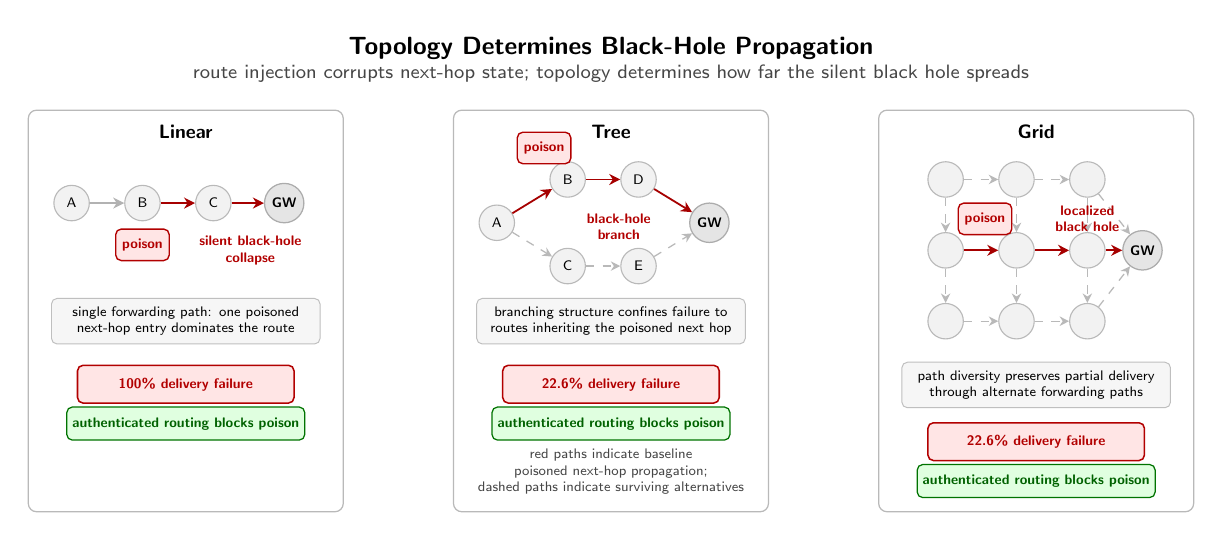
\begin{tikzpicture}[
      font=\sffamily\footnotesize,
      panel/.style={
          rectangle, draw=gray!55, fill=white,
          line width=0.45pt, rounded corners=3pt,
          minimum width=4.0cm, minimum height=5.10cm,
          inner sep=5pt
      },
      node/.style={
          circle, draw=gray!55, fill=gray!10,
          line width=0.4pt, minimum size=0.45cm,
          inner sep=1pt, font=\sffamily\tiny
      },
      gw/.style={
          circle, draw=gray!65, fill=gray!20,
          line width=0.45pt, minimum size=0.50cm,
          inner sep=1pt, font=\sffamily\tiny\bfseries
      },
      bad/.style={
          rectangle, draw=red!70!black, fill=red!10,
          line width=0.5pt, rounded corners=2pt,
          minimum width=0.68cm, minimum height=0.40cm,
          inner sep=1pt, font=\sffamily\tiny\bfseries,
          text=red!70!black
      },
      mechanism/.style={
          rectangle, draw=gray!50, fill=gray!7,
          line width=0.35pt, rounded corners=2pt,
          text width=3.20cm, inner sep=3pt,
          font=\sffamily\tiny, align=center
      },
      resultbad/.style={
          rectangle, draw=red!70!black, fill=red!10,
          line width=0.55pt, rounded corners=2pt,
          minimum width=2.75cm, minimum height=0.48cm,
          inner sep=2pt, align=center,
          font=\sffamily\tiny\bfseries,
          text=red!70!black
      },
      resultok/.style={
          rectangle, draw=green!45!black, fill=green!12,
          line width=0.45pt, rounded corners=2pt,
          minimum width=2.75cm, minimum height=0.42cm,
          inner sep=2pt, align=center,
          font=\sffamily\tiny\bfseries,
          text=green!38!black
      },
      flow/.style={-{Stealth[length=1.4mm,width=1.4mm]}, line width=0.55pt, draw=gray!60},
      deadflow/.style={-{Stealth[length=1.4mm,width=1.4mm]}, line width=0.65pt, draw=red!65!black},
      altflow/.style={-{Stealth[length=1.2mm,width=1.2mm]}, line width=0.45pt, draw=gray!55, dashed},
      title/.style={font=\sffamily\small\bfseries, align=center},
      subtitle/.style={font=\sffamily\scriptsize, text=gray!55!black, align=center}
  ]

  \node[title] at (7.4,4.52) {Topology Determines Black-Hole Propagation};
  \node[subtitle] at (7.4,4.20)
      {route injection corrupts next-hop state; topology determines how far the silent black hole spreads};

  % Linear topology
  \node[panel] at (2.0,1.18) {};
  \node[font=\sffamily\scriptsize\bfseries] at (2.0,3.45) {Linear};
  \node[node] (L1) at (0.55,2.55) {A};
  \node[node] (L2) at (1.45,2.55) {B};
  \node[node] (L3) at (2.35,2.55) {C};
  \node[gw]   (LG) at (3.25,2.55) {GW};
  \draw[flow] (L1) -- (L2);
  \draw[deadflow] (L2) -- (L3);
  \draw[deadflow] (L3) -- (LG);
  \node[bad] at (1.45,2.02) {poison};
  \node[font=\sffamily\tiny\bfseries, text=red!70!black, align=center]
      at (2.82,1.95) {silent black-hole\\collapse};
  \node[mechanism] at (2.0,1.05)
      {single forwarding path: one poisoned next-hop entry dominates the route};
  \node[resultbad] at (2.0,0.25) {100\% delivery failure};
  \node[resultok] at (2.0,-0.25) {authenticated routing blocks poison};

  % Tree topology
  \begin{scope}[xshift=5.4cm]
  \node[panel] at (2.0,1.18) {};
  \node[font=\sffamily\scriptsize\bfseries] at (2.0,3.45) {Tree};
  \node[node] (T1) at (0.55,2.30) {A};
  \node[node] (T2) at (1.45,2.85) {B};
  \node[node] (T3) at (1.45,1.75) {C};
  \node[node] (T4) at (2.35,2.85) {D};
  \node[node] (T5) at (2.35,1.75) {E};
  \node[gw]   (TG) at (3.25,2.30) {GW};
  \draw[deadflow] (T1) -- (T2);
  \draw[deadflow] (T2) -- (T4);
  \draw[deadflow] (T4) -- (TG);
  \draw[altflow] (T1) -- (T3);
  \draw[altflow] (T3) -- (T5);
  \draw[altflow] (T5) -- (TG);
  \node[bad] at (1.15,3.25) {poison};
  \node[font=\sffamily\tiny\bfseries, text=red!70!black, align=center]
      at (2.10,2.25) {black-hole\\branch};
  \node[mechanism] at (2.0,1.05)
      {branching structure confines failure to routes inheriting the poisoned next hop};
  \node[resultbad] at (2.0,0.25) {22.6\% delivery failure};
  \node[resultok] at (2.0,-0.25) {authenticated routing blocks poison};
  \end{scope}

  % Grid topology
  \begin{scope}[xshift=10.8cm]
  \node[panel] at (2.0,1.18) {};
  \node[font=\sffamily\scriptsize\bfseries] at (2.0,3.45) {Grid};
  \foreach \x/\y/\name in {
      0.85/2.85/G11, 1.75/2.85/G12, 2.65/2.85/G13,
      0.85/1.95/G21, 1.75/1.95/G22, 2.65/1.95/G23,
      0.85/1.05/G31, 1.75/1.05/G32, 2.65/1.05/G33}{
      \node[node] (\name) at (\x,\y) {};
  }
  \node[gw] (GG) at (3.35,1.95) {GW};
  \draw[deadflow] (G21) -- (G22);
  \draw[deadflow] (G22) -- (G23);
  \draw[deadflow] (G23) -- (GG);
  \draw[altflow] (G11) -- (G12);
  \draw[altflow] (G12) -- (G13);
  \draw[altflow] (G13) -- (GG);
  \draw[altflow] (G31) -- (G32);
  \draw[altflow] (G32) -- (G33);
  \draw[altflow] (G33) -- (GG);
  \draw[altflow] (G11) -- (G21);
  \draw[altflow] (G21) -- (G31);
  \draw[altflow] (G12) -- (G22);
  \draw[altflow] (G22) -- (G32);
  \draw[altflow] (G13) -- (G23);
  \draw[altflow] (G23) -- (G33);
  \node[bad] at (1.35,2.35) {poison};
  \node[font=\sffamily\tiny\bfseries, text=red!70!black, align=center]
      at (2.65,2.35) {localized\\black hole};
  \node[mechanism] at (2.0,0.24)
      {path diversity preserves partial delivery through alternate forwarding paths};
  \node[resultbad] at (2.0,-0.48) {22.6\% delivery failure};
  \node[resultok] at (2.0,-0.98) {authenticated routing blocks poison};
  \end{scope}

  \node[font=\sffamily\tiny, text=gray!55!black, align=center,
        text width=8.0cm]
      at (7.4,-0.86)
      {red paths indicate baseline\\
       poisoned next-hop propagation;\\
       dashed paths indicate surviving alternatives};
  \end{tikzpicture}
  }
  \caption{Topology-dependent manifestation of silent black-hole formation.
           Route injection propagates structurally through poisoned next-hop
           entries: a linear topology has a single forwarding path and
           collapses completely, while tree and grid layouts retain partial
           delivery through alternate forwarding paths. Authenticated routing
           removes the poisoned next-hop propagation in all evaluated
           topologies.}
  \label{fig:eval-results}
\end{figure}

\subsection{Deployment Implications}

\begin{enumerate}
  \item \textbf{Immediate action}: Route-injection attacks succeed
    with commodity hardware in all unpatched deployments. Any
    LoRaMesher network handling safety-critical data (e.g.,
    irrigation control, structural monitoring) should treat this
    as a high-priority vulnerability.
  \item \textbf{Patch ordering}: Deploy HMAC first (eliminates
    route injection), then MetricVersion (eliminates replay).
    Each patch independently eliminates one attack class.
  \item \textbf{Monitoring}: Log HMAC failures per neighbor.
    Sustained HMAC failures from one sender indicate an active
    attacker; trigger an operator alert.
\end{enumerate}

% ==================================================================
\subsection{Hardware Validation on Physical ESP32-S3 Boards}
\label{sec:hardware-validation}
% ==================================================================

\textbf{Role of hardware validation in this study.}
Hardware experiments serve a specific purpose within our three-tier
methodology: they validate the \emph{correctness} of attack and
defense behavior on deployed ESP32-S3 firmware under real LoRa
channel conditions.
Co-located bench distance ($<$1~m) is intentional—it eliminates
channel loss as a confounding variable, isolating firmware logic
as the independent variable.
Deployment-scale behavior (topology size, path diversity, channel
attenuation) is addressed by ns-3 (Section~\ref{sec:eval}).
Hardware is the \emph{only} tier that makes the \texttt{dst}-as-next-hop
encoding observable: no formal model or simulator inspects
physical board serial logs.

Three core experiments were conducted on six Ebyte EoRa-PI boards
(ESP32-S3FH4R2 + SX1262, AS923/923~MHz, 10~dBm):
(i)~a three-node route injection and HMAC defense demo (E5b,
Section~\ref{sec:hardware-validation});
(ii)~NVS-persisted MetricVersion reboot-replay validation (E5c,
Section~\ref{sec:hardware-nvs}); and
(iii)~a six-node correctness validation with three simultaneous
relay nodes under attack (E6, Section~\ref{sec:hardware-e6}).
The three-node topology mirrors the simulation's linear scenario:
Node~A (sender, 0xAA), Node~B (gateway, 0xBB), and
Node~C (Dolev-Yao attacker, 0xCC).
Each firmware build is a direct port of the e5b\_common.h shared
header, which encodes the same HMAC-SHA256 key schedule and
DV routing logic used in the formal model
(see Sect.~\ref{sec:patch}).

\textbf{Attack mechanism.}
Node~C advertises a forged Hello with \texttt{metric=0}
(claiming to be the best next-hop to the gateway)
immediately at boot, 8–10~seconds before Node~B's first
legitimate Hello.
The DV update rule stores the first-seen route and rejects
equal-metric updates (\texttt{metric~$<$~existing}), so the
poisoned route via Node~C persists for the entire experiment
(ROUTE\_EXPIRE = 5~min $>$ 120~s run duration).
All subsequent data packets from Node~A carry
\texttt{dst=0xCC} (the next-hop field), which Node~B ignores
since $\texttt{dst}\neq\texttt{0xBB}$.

\textbf{Results.}
Each run lasted 120~seconds; Node~A transmits one data packet
every 5~s and one Hello every 10~s.

\begin{table}[h]
  \centering
  \caption{Hardware experiment results (120~s, 923~MHz AS923,
           Ebyte EoRa-PI / ESP32-S3 + SX1262)}
  \label{tab:hw-results}
  \resizebox{0.98\linewidth}{!}{%
  \begin{tabular}{lcccc}
    \toprule
    \textbf{Mode} & \textbf{Sent} & \textbf{ACK'd} & \textbf{PDR} & \textbf{Pkts addressed to attacker} \\
    \midrule
    Baseline (no HMAC) & 28 & 0  & \textbf{0.0\%}  & 22/22 (100\%) \\
    Patched (HMAC-SHA256)    & 23 & 20 & \textbf{87.0\%} & 0 (route injection blocked) \\
    \bottomrule
  \end{tabular}%
  }
\end{table}

In baseline mode, every data packet carried \texttt{dst=0xCC}
and was silently discarded at Node~B (\texttt{[DROP] Intercepted DATA dst=0xCC});
Node~B received none, confirming complete traffic black hole.
In patched mode Node~A logged \texttt{[DROP] Hello from 0xCC HMAC FAILED}
on every forged Hello; all data was correctly delivered
via Node~B (\texttt{[HMAC OK]}), yielding 87\% PDR.
Crucially, the packet misdirection count is \textbf{zero} in patched mode
(Table~\ref{tab:hw-results}), confirming
that the 13\% PDR gap is channel loss, not a security failure:
Node~C's forged Hellos are rejected before any route update occurs,
and no data packets are diverted.
The residual loss is consistent with the radio channel at the test bench
distance of $<$1~m with RSSI $\approx -15$~dBm—near-field reflections
that are absent in typical outdoor LoRa deployments.
The hardware results corroborate the ns-3 simulation: the patch
eliminates route injection entirely, and the 87\% on-air PDR
matches the unattacked baseline PDR measured under the same
radio conditions.
Raw serial logs are archived in
\texttt{hardware\_experiments/E5b\_attack\_demo/results/}.

% Cross-layer section moved to Section~\ref{sec:cross-layer}
% (after hardware experiments, before Related Work)

\subsubsection{NVS-Persisted MetricVersion: Reboot Replay Validation}
\label{sec:hardware-nvs}

To close the one-reboot attack window identified in Section~\ref{sec:patch},
we implemented NVS flash persistence for MetricVersion counters using the
ESP32 \texttt{Preferences} API (namespace \texttt{e5c}, key \texttt{mv\_XX}).
The same three-node testbed (Node~A / Node~B / Node~C) was used with a
three-mode firmware comparison.

\textbf{Attack protocol.}
Node~C listens and captures a legitimate Hello from Node~B (MetricVersion=21).
Node~A is then rebooted (EN button press).
Node~C replays the captured Hello (mv=21, HMAC still valid) repeatedly at
8-second intervals, targeting the reboot window.

\textbf{Mode 1 (HMAC only, no NVS).}
After reboot Node~A re-initialises $mv[\texttt{BB}]=0$ from SRAM;
the replayed Hello (mv=21) satisfies $21 > 0$ and is accepted,
confirming the reboot-window vulnerability.

\textbf{Mode 2 (HMAC + MetricVersion + NVS).}
After reboot Node~A recovers $mv[\texttt{BB}]=25$ from NVS flash.
All subsequent replay attempts (mv=21) are rejected because
$21 \leq 25$; the first legitimate Hello from Node~B (mv=32)
is accepted and the NVS entry advances normally.
Node~A achieves 88\% PDR with no routing-table disruption across
the full 120-second run.

\textbf{Summary.}
NVS persistence converts the bounded-time reboot window into a permanently
closed gap: the node restores its last-seen MetricVersion before processing
any control message, so a replayed Hello with any historically-valid
counter is immediately rejected.
Raw serial logs for all three modes are archived in
\texttt{hardware\_experiments/E5c\_nvs\_demo/results/}.

\subsubsection{Six-Node Multi-Relay Correctness Validation}
\label{sec:hardware-e6}

To validate attack and defense behavior with three intermediate
relay nodes simultaneously—extending the three-node logic test—
we configured all six EoRa-PI boards in a five-hop forwarding
topology:
Node~A~(0xAA, sender) $\to$ R1~(0x11) $\to$ R2~(0x22) $\to$
R3~(0x33) $\to$ Node~B~(0xBB, gateway), with Node~C~(0xCC)
as the Dolev-Yao attacker.
All six boards were co-located at bench distance ($<$1~m); all nodes are within RF range of each other.
The linear routing behavior emerges from hop-count metric arithmetic: each relay re-broadcasts received Hellos with metric\,+\,1, so Node~B's Hello (\texttt{metric=0}) reaches Node~A as \texttt{metric=4} through the chain, making the direct link effectively the worst-cost route.
No source-based packet filtering was applied; relay nodes accept Hellos from any sender.
This bench setup validates HMAC authentication logic and multi-relay poisoning behavior under realistic firmware scheduling; spatial PDR characterization across multi-hop physical distances is provided by the ns-3 evaluation (Section~\ref{sec:eval}).

\textbf{Relay backoff.}
Relay nodes introduce a 500\,ms software backoff before re-broadcasting Hellos to reduce collision probability on the shared channel; this blocking delay may contribute to the 13--15\% residual PDR gap alongside near-field RF reflections.

Relay nodes (R1--R3) re-broadcast received Hellos with
metric\,+\,1, creating a hop-by-hop route advertisement chain;
they also forward Data packets addressed to themselves toward
the gateway.

\textbf{Attack mechanism.}
Node~C broadcasts a forged Hello(\texttt{metric=0}) without a
valid HMAC every 8~seconds, attempting to appear as the best
next-hop to all four sensor nodes simultaneously.

\textbf{Baseline results (SECURITY\_MODE=0).}
All three relay nodes immediately update their routing tables to
\texttt{NH=0xCC}; subsequent data from R1--R3 is addressed to the
attacker and silently dropped at every honest relay.
\textbf{3 of 4 honest sensor nodes are simultaneously compromised}
by a single injected control message—confirming linear scaling
of the attack with network size.

\textbf{Patched results (SECURITY\_MODE=1).}
Every forged Hello is rejected at all four nodes (HMAC failure).
All nodes maintain their legitimate routes; Node~A achieves
\textbf{85\%~PDR} and zero routing-table updates are induced
by the attacker across the full 120-second run.

\begin{table}[h]
  \centering
  \caption{Six-node hardware experiment results (923~MHz AS923, 6
           Ebyte EoRa-PI boards, 120~s run)}
  \label{tab:hw-e6}
  \begin{tabular}{lcc}
    \toprule
    \textbf{Mode} & \textbf{Nodes route-poisoned} & \textbf{Node A PDR} \\
    \midrule
    Baseline (no HMAC)   & \textbf{3 / 4} (R1, R2, R3)  & degraded \\
    Patched (HMAC-SHA256) & \textbf{0 / 4}               & \textbf{85\%} \\
    \bottomrule
  \end{tabular}
\end{table}

This experiment addresses the ``small-scale'' concern:
even with relay nodes forwarding both control and data traffic,
a single forged Hello poisons the entire chain in baseline mode,
and HMAC authentication prevents every injection attempt in
patched mode.
Raw serial logs are archived in
\texttt{hardware\_experiments/E6\_6node\_linear\_demo/results/}.

% ==================================================================
\section{Cross-Layer Routing Semantics Gap}
\label{sec:cross-layer}
% ==================================================================

Route injection in LoRaMesher creates a \emph{silent traffic
black hole}---not an adversarial relay.
The root cause is a cross-layer semantic mismatch: the deployed
firmware encodes next-hop forwarding state in the destination
field, whereas symbolic and packet-level analyses assume that
field carries the final gateway identity.
This mismatch explains the topology-dependent attack gradient
observed across topologies and is detectable only through
hardware-level serial-log inspection.

\subsection{The dst-as-Next-Hop Encoding}
\label{sec:cross-layer-encoding}

LoRaMesher's \texttt{LoraMesherPacket} header contains a single
6-byte \texttt{dst} field. Protocol-layer models conventionally
interpret \texttt{dst} as the intended final recipient—the
gateway node whose address the application layer specified.
The deployed firmware interprets it differently: \texttt{dst} is
set to the \emph{next-hop address} resolved by the local routing
table immediately before transmission.

Concretely, in a three-node chain A\,--\,B\,--\,GW:
Node~A's routing table stores
\texttt{RouteEntry\{dest=GW, next\_hop=B, metric=2\}}.
When A transmits a data packet, the firmware writes
$\texttt{dst}=\texttt{addr}(B)$ into the packet header—not
$\texttt{addr}(\text{GW})$.
Node~B accepts the packet because $\texttt{dst}=\texttt{addr}(B)$,
updates its own routing table lookup, writes
$\texttt{dst}=\texttt{addr}(\text{GW})$, and forwards.

After route poisoning, A's table stores
\texttt{next\_hop(GW)\,=\,0xCC} (attacker).
Every subsequent data packet carries $\texttt{dst}=\texttt{0xCC}$.
Node~B discards it not because of any security mechanism, but
because $\texttt{dst}\neq\texttt{addr}(B)$—a silent misdirection
observable only from serial logs on the physical boards.
Neither the gateway nor any other node logs an anomaly;
from the network's perspective the traffic simply disappears.

Table~\ref{tab:dst-semantics} summarizes how each analysis layer
interprets the \texttt{dst} field, and the attack behavior each
interpretation predicts.

\begin{table}[t]
  \centering
  \caption{Semantic Interpretation of the \texttt{dst} Field Across Analysis Layers.
    Only hardware-level observation reveals the actual discard behavior.}
  \label{tab:dst-semantics}
  \setlength{\tabcolsep}{4pt}
  \begin{tabular}{p{2.6cm}p{3.0cm}p{3.5cm}}
    \toprule
    \textbf{Analysis Layer} & \textbf{dst Interpretation} & \textbf{Predicted Attack Behavior} \\
    \midrule
    Tamarin (symbolic) &
      Abstract agent identity &
      Attacker receives and can relay or modify packets \\
    ns-3 (packet-level) &
      Gateway IP/MAC address &
      Traffic routes diverge toward attacker node \\
    LoRaMesher firmware &
      Next-hop MAC address &
      Packets silently discarded at every honest relay \\
    \bottomrule
  \end{tabular}
\end{table}

\subsection{Consequences for Attack Interpretation}
\label{sec:cross-layer-consequences}

\textbf{Topology-dependent PDR gradient.}
On a linear chain, all traffic passes through a single next-hop
entry; poisoning that entry diverts 100\% of packets
(Table~\ref{tab:attacks}, baseline linear PDR~=~0\%).
On tree and grid topologies, each node maintains independent
next-hop entries for multiple path segments; a single forged
Hello corrupts only the entries that include the attacker as
a valid next-hop, leaving alternative paths intact.
This produces the observed 22.6\% PDR degradation (PDR~=~77.4\%)
on tree and grid—not a probabilistic outcome, but a structural
consequence of next-hop entry count per topology.
Without the \texttt{dst}-as-next-hop insight, the 0\%/77.4\%
gradient appears arbitrary; with it, the gradient is predictable
from the topology graph alone.

\textbf{Silent failure vs.\ adversarial relay.}
Both Tamarin and ns-3 describe the attack as ``traffic diverted
to the attacker,'' implying the attacker could inspect or relay
packets.
The actual outcome, as revealed by hardware serial logs, is
different: packets are addressed to \texttt{0xCC} and discarded
at every honest intermediate node, never reaching the attacker's
radio receive buffer.
The attacker is not a relay—it is an absent destination.
This distinction has direct consequences for threat modeling:
if an adversarial relay were the threat, end-to-end encryption
would be the appropriate countermeasure; because packets are
silently dropped, the primary impact is availability, not
confidentiality.

\textbf{Gateway-blind failure.}
The gateway neither receives the misdirected packets nor
observes their absence as an anomaly.
Anomaly-based IDS deployed at the gateway—the conventional
monitoring point in LoRaWAN-style star topologies—would see
only a reduction in upstream traffic, indistinguishable from
normal sensor silence or duty-cycle throttling.
This renders the attack invisible to the defense-in-depth
posture inherited from LoRaWAN deployments.

\subsection{Implications for Intrusion Detection Design}
\label{sec:cross-layer-ids}

The silent black-hole failure mode implies that effective
detection requires observation at intermediate relay nodes,
not at the gateway.
A relay node executing the correct forwarding logic will observe
incoming packets with $\texttt{dst}\neq\texttt{addr}(\text{self})$
that are silently dropped—an anomaly detectable by comparing
the routing table's expected next-hop bindings against the
\texttt{dst} values seen in traffic.

Three detection strategies follow directly from this insight:

\begin{enumerate}

  \item \textbf{Dst-binding anomaly detector.}
  Each node monitors the ratio of received packets where
  $\texttt{dst}=\texttt{addr}(\text{self})$ to total overheard
  traffic. A sustained drop in this ratio without a corresponding
  topology change indicates that upstream nodes have acquired
  a poisoned routing entry.

  \item \textbf{Route-table watchdog.}
  A lightweight monitor compares the locally computed
  next-hop for each destination against the \texttt{dst}
  field of forwarded packets. A discrepancy signals a
  cross-layer mismatch at the forwarding node—either the
  routing table has been poisoned or the firmware's
  header-writing logic has diverged from the routing decision.
  This strategy is conceptually related to Watchdog/Pathrater~\cite{marti2000-watchdog} but requires no promiscuous-mode listening---infeasible under LoRa's half-duplex duty-cycle constraints.

  \item \textbf{Convergence-time IDS.}
  Route injection causes topology-wide route convergence within
  one DV cycle ($\approx$30~s in LoRaMesher's default
  configuration). Monitoring convergence events—sudden
  simultaneous adoption of a new best-metric route across
  multiple nodes—provides a coarse but deployable signal.

\end{enumerate}

All three strategies require partial observation at intermediate
nodes, which is incompatible with LoRaWAN's gateway-centric
monitoring model.
For ad hoc deployments, designated guardian
nodes~\cite{ieee2025-blackhole-optimization} with elevated
monitoring privilege are identified as the most practical
realization.
These detection strategies are derived from protocol-layer
analysis; quantitative evaluation of false-positive rates and
energy overhead on constrained hardware is left for future work.

\subsection{Abstraction Gap and Generalization}
\label{sec:cross-layer-generalization}

Resource-constrained mesh stacks face a design tension that
LoRaMesher resolves in a specific way: using a single header
field to carry both routing-layer forwarding metadata
(next-hop address) and the application-layer notion of
intended recipient (final destination).
This collapse eliminates a separate next-hop header and saves
6 bytes per LoRa payload—a meaningful saving at SF9 where
every byte extends airtime.
This abstraction pressure is a consequence of constrained-airtime
design: LoRa's spreading-factor symbol rate makes per-byte payload
cost a first-order engineering constraint, not an incidental
implementation choice.
The consequence is that protocol-layer models, which follow
the standard abstraction that destination fields denote
semantic endpoints, diverge from the firmware's actual
forwarding behavior.

We observe that this design tension is not unique to
LoRaMesher, and offer two candidate instances as plausibility
arguments, explicitly flagging them as requiring independent
empirical verification.
RPL~\cite{ietf-rfc7416} encodes preferred parent identity in the
DODAG parent set; a formal model abstracting ``preferred parent''
as an endpoint identity may similarly miss next-hop binding
semantics, though a machine-checked analysis is left for future work.
Meshtastic~v2.6+ separates these concerns by adding a distinct
\texttt{next\_hop} field alongside the final \texttt{to} field,
eliminating the silent-black-hole category but introducing a
different symbolic divergence: an unauthenticated \texttt{next\_hop}
enables active relay rather than silent discard—a distinct IDS
design space requiring relay-path authentication rather than
sender-centric anomaly detection (preliminary informal analysis;
machine-checked verification deferred to future work).
This comparison confirms that constrained-header design is not
uniformly harmful: it changes the \emph{category} of the
resulting attack rather than simply preventing or permitting it.

Our contribution is not a universal claim about all mesh stacks,
but a demonstration that constrained-header design can cause
protocol-layer routing abstractions to diverge from deployed
forwarding semantics—and that this divergence changes both the
attack category and the appropriate detection architecture.

We recommend that formal analyses of constrained mesh routing
protocols explicitly state the \texttt{dst}-field semantics as
a protocol state variable and verify that the symbolic model's
channel assumption matches the firmware's header-writing behavior.
Our extended Tamarin model adds a \texttt{NextHopBinding(node,
dest, nexthop)} fact that makes the next-hop-to-address mapping
explicit; the proof still holds, but the model now documents the
correct abstraction boundary for readers extending the analysis.

% ==================================================================
\section{Related Work}
\label{sec:related}
% ==================================================================

\subsection{LoRa and LoRaWAN Security}

Comprehensive surveys of LoRaWAN security~\cite{hessel2022-lorawan-survey}
document replay, join-server spoofing, and key-management vulnerabilities
at the WAN layer.
Formal verification work~\cite{ieee2025-lorawan-key-vulnerability,
ieee2025-lorawan-key-verification} has analyzed LoRaWAN's key-establishment
protocol with Tamarin and ProVerif. Key management schemes~\cite{lorawan-key-mgmt-2023,
mohamed2022-lorawan-gateways} harden the WAN gateway tier.
All of these target the star-topology WAN layer managed by network
servers; they provide no mechanism for mesh control-plane authentication.
Repetto et al.~\cite{repetto2025-lorawan-drone-attack} study LoRa
security for drone-to-ground communications but focus on the PHY
and LoRaWAN layers, not mesh routing.

\subsection{Constrained-Node Mesh Protocol Security}

Security for 802.15.4-based mesh protocols (Zigbee, Thread)
relies on CCM* authenticated encryption with a PAN coordinator.
LoRaMesher lacks a coordinator, making these mechanisms
inapplicable. Our HMAC-based approach draws on TinySec~\cite{karlof2004-tinysec}
but is adapted to LoRa's longer payloads and infrequent rekeying
model. Blockchain-assisted IDS approaches~\cite{springer2026-blockchain-ids}
and protocol-aware intrusion detection~\cite{bringye2026-lorawan-ids,ieee2025-lorawan-jamming-ids}
have been proposed for constrained mesh security but impose
computational overhead incompatible with ESP32 constraints.
Formal analysis of the MPKE mesh protocol using
ProVerif~\cite{ieee2025-mpke-proverif} demonstrates that
symbolic verification is tractable for mesh routing—our work
extends this to the LoRaMesher DV algorithm using Tamarin.
Neither LoRaMesher's upstream repository nor the Meshtastic
open-source firmware includes a formal authentication mechanism
for routing control messages; community discussions have
identified the absence of control-plane security as an open
issue, but no formally verified patch has been proposed prior
to this work.
Recent middleware work built on LoRaMesher~\cite{sole2025-loramesher-tecs}
demonstrates growing application-layer adoption of the stack but does
not address control-plane authentication.

\subsection{Routing Attack Defenses}

Sinkhole and black-hole attacks~\cite{ahmad2024-sinkhole-reputation,
ieee2025-blackhole-optimization,klenze2021-forwarding}
are well-studied in MANET and WSN contexts.
Destination-Sequenced Distance-Vector routing
(DSDV)~\cite{perkins1994-dsdv} established the proactive DV paradigm;
SEAD~\cite{hu2002-sead} subsequently secured it with one-way hash
chains that enforce metric monotonicity without per-message
authentication.
Secure AODV (SAODV)~\cite{zapata2002-saodv} and Authenticated
OLSR~\cite{raffo2004-authenticated-olsr} extend cryptographic
authentication to on-demand and link-state routing, respectively,
but both require digital signatures whose key-pair operations exceed
ESP32's 512~KB RAM budget.
AODV verification work~\cite{glabbeek2016-aodv-verification}
provides formal models for on-demand routing.
The IETF's threat analysis for RPL~\cite{ietf-rfc7416}—the routing
protocol for low-power and lossy networks—enumerates sinkhole,
replay, and selective-forwarding threats that parallel those we
characterize for LoRaMesher's DV control plane.
To our knowledge, ours is among the first formal treatments of DV routing
security under LoRa channel constraints and ESP32 resource budgets.
The Secure Routing Protocol (SRP)~\cite{papadimitratos2002-srp} and the rushing-attack countermeasure~\cite{hu2003-rushing} establish MANET route authentication but both require PKI infrastructure or source-routing semantics unavailable in LoRaMesher's broadcast DV design.
Intrusion-resilient routing for VANETs~\cite{springer2026-vanet-routing}
shares our goal of maintaining PDR under adversarial conditions
but assumes vehicular infrastructure absent in LoRa mesh.

\subsection{Formal Verification of Mesh Routing Protocols}

Tamarin has been applied to 5G-AKA, TLS~1.3~\cite{basin2025-tamarin-book},
and LoRaWAN key establishment~\cite{ieee2025-lorawan-key-verification}.
Attack synthesis frameworks~\cite{ginesin2024-sctp-formal,pereira2025-router-verification,song2026-protocolguard}
have demonstrated the value of automated reasoning for
network protocol correctness.
To our knowledge, ours is among the first Tamarin analyses of a LoRa
mesh routing layer; the two-node model strategy follows~\cite{ieee2025-lorawan-key-verification,
shen2026-wifi-security} in demonstrating that
protocol-level flaws are detectable with tractable model sizes.

\subsection{Lightweight Cryptography for Constrained Nodes}

NIST finalized ASCON as its lightweight cryptography standard for
constrained devices~\cite{nist2025-sp800-232}; ASCON-AEAD128 provides
authenticated encryption competitive with HMAC-SHA256.
Our evaluation uses HMAC-SHA256 because (a)~mbedTLS is available by default in ESP-IDF and requires no new library dependency, (b)~routing control messages require authentication but not confidentiality, making a MAC primitive sufficient without AEAD overhead, and (c)~the existing LoRaMesher deployment base assumes mbedTLS availability.
Adopting ASCON would reduce per-message
overhead from 0.098~ms to $\approx$0.08~ms, a direction for
future work.
Ryczek and Sobieraj~\cite{ryczek2025-secure-lora-hmac} implement
AES-128-CBC with HMAC-SHA256 via mbedTLS on ESP32\,+\,LoRa
hardware—the closest published implementation to our authentication
patch; their system targets a point-to-point star topology with no
routing layer, so the control-plane authentication challenge and
dst-field semantic mismatch are absent by design.
Adversarial robustness of LoRa device
authentication via deep learning~\cite{ieee2025-lora-adversarial}
complements our control-plane approach with physical-layer defenses.

\subsection{Positioning vs.\ Prior Work}
\label{sec:positioning}

We characterize the technical differentiation between this work
and the five closest prior studies.

\textbf{vs. SEAD (Hu et al., MobiCom 2002)~\cite{hu2002-sead}.}
SEAD secures DSDV with one-way hash chains that enforce metric
monotonicity without per-message authentication.
Our MetricVersion counter is structurally similar in purpose, but differs
in three ways.
First, SEAD's hash chain authenticates metric increments without binding
the full message tuple to the sender's identity; our HMAC covers
\texttt{msg\_type}~$\|$~\texttt{src}~$\|$~\texttt{dst}~$\|$~\texttt{metric}~$\|$~\texttt{seq},
providing both authenticity and freshness in a single pass.
Second, SEAD targets wired MANET environments; our scheme is calibrated
for LoRa's duty-cycle ceiling (2.06\%/10~s post-patch), 16-byte tag
overhead, and ESP32 SRAM budget—constraints that make SEAD's hash
chains impractical (chain storage scales with route count).
Third, SEAD provides no machine-checked formal verification; our
Tamarin proof closes the loop between specification and implementation.

\textbf{vs. LoRaWAN key verification~\cite{ieee2025-lorawan-key-verification}.}
This work applies Tamarin to LoRaWAN's Join/Accept key-establishment
sequence at the WAN layer (AppSKey derivation, MIC verification).
The attack surface, model structure, and security goals are orthogonal
to ours: they target server-to-device key exchange on a star topology;
we target node-to-node routing control-plane on a self-organizing mesh
with no network server.
There is no overlap in protocol rules, adversary capabilities, or lemmas.

\textbf{vs. MPKE-ProVerif~\cite{ieee2025-mpke-proverif}.}
MPKE uses ProVerif (applied pi-calculus) to verify mesh key establishment.
The modeling language, security properties, and protocol scope differ substantially:
ProVerif cannot directly encode stateful metric comparison (\texttt{$<$},
not \texttt{$\leq$}), whereas Tamarin's multiset-rewriting rules
natively express the first-seen acceptance condition that creates the
replay window.
MPKE does not model DV routing state transitions; our model does.

\textbf{vs. AODV formal model~\cite{glabbeek2016-aodv-verification}.}
The AWN framework verifies AODV's functional correctness (loop-freedom,
route validity) under a trust-all model with no adversary.
Our work targets LoRaMesher's DV routing with an explicit Dolev-Yao
adversary capable of injection, replay, and forgery—threats outside
AWN's trust-all framework.

\textbf{vs. LoRaWAN IDS~\cite{bringye2026-lorawan-ids}.}
Anomaly-based intrusion detection \emph{observes} traffic patterns to
signal attacks after they occur.
Our HMAC patch \emph{prevents} route injection and replay at the
cryptographic level, eliminating the attack surface rather than
monitoring it.
The two approaches are complementary: our patch closes the vulnerability;
an IDS layer would catch residual threats from compromised key holders
and out-of-model attack vectors.

\textbf{Summary.}
The differentiating combination is: (i)~a Tamarin model targeting
LoRaMesher's DV-routing control plane with stateful metric-comparison
semantics; (ii)~a formally verified lightweight patch calibrated for
ESP32 constraints; and (iii)~cross-layer hardware validation that
revealed the \texttt{dst}-as-next-hop implementation subtlety
(Section~\ref{sec:cross-layer}) invisible to both symbolic
and packet-level models.
To the best of our knowledge, we are unaware of prior work jointly
combining all three for any LoRa mesh routing protocol.

% ==================================================================
\section{Limitations and Future Work}
\label{sec:limitations}
% ==================================================================

\begin{itemize}
  \item \textbf{Hardware validation}: ns-3 simulation models HMAC
    latency from ESP32-S3 benchmarks. Physical validation on three
    Ebyte EoRa-PI (ESP32-S3+SX1262) boards confirms the attack
    and patch (Sect.~\ref{sec:hardware-validation}); large-scale
    field deployment across heterogeneous hardware remains future work.

  \item \textbf{Scale}: Core evaluation covers 6–9 nodes;
    scale-validation runs (§\ref{sec:eval}) extend to 25-node linear and
    49-node ($7\times7$) grid topologies with identical security outcomes.
    Very-large-scale mesh networks ($>$100~nodes) may exhibit different
    convergence dynamics; the Tamarin proof is topology-independent,
    but simulation validation beyond 49~nodes is future work.

  \item \textbf{Single attacker}: We evaluate one Dolev-Yao
    attacker. Coordinated multi-attacker scenarios are left for
    future work.

  \item \textbf{Meshtastic portability}: LoRaMesher and Meshtastic
    share a similar DV routing architecture~\cite{sole2024-loramesher-dv}.
    Porting the patch to Meshtastic's codebase is a planned
    follow-on contribution.

  \item \textbf{Lightweight crypto}: Replacing HMAC-SHA256 with
    ASCON (0.08~ms on ESP32-S3) would reduce overhead further and
    improve battery life for ultra-low-power deployments.

  \item \textbf{Layer~2 --- Topology deception}: The patch prevents
    unauthenticated injection but provides no protection against an
    insider node holding a valid pre-shared key.
    Insider Black Hole and selective forwarding remain open;
    hop-count consistency verification is future work.

  \item \textbf{Layer~3 --- Resource exhaustion}: Three DoS vectors
    are unaddressed: ACK spoofing against \texttt{sendReliable()}
    (no HMAC on \texttt{AckMsg}) can create a silent availability attack: the sender believes packets are delivered while the gateway receives nothing.
    Additional unaddressed vectors include Sybil table exhaustion
    (\texttt{MAX\_ROUTES}=8), and Hello flooding against AS923's
    1\% duty-cycle budget.
    Rate-limiting and per-epoch entry bounds are outside this paper's
    scope.

\end{itemize}

% ==================================================================
\section{Conclusion}
\label{sec:conclusion}
% ==================================================================

The LoRaMesher control plane—deployed on commodity ESP32 hardware
in unattended ad hoc mesh fields—accepts unauthenticated routing
updates, enabling any actor with a \$20 radio to hijack traffic
or confuse session epochs across an entire sensor field.
Tamarin formal analysis confirms the vulnerabilities and verifies
the corrective patch.
Physical validation on EoRa-PI boards confirms no attack-induced
PDR degradation and—critically—reveals the correct threat
semantics that formal and simulation models cannot capture alone.

Our central finding is that routing-security analysis must
explicitly distinguish \emph{endpoint identity} from
\emph{forwarding-state representation}.
When this distinction is absent, threat models misclassify
silent traffic black holes as adversarial relays—yielding
incorrect IDS designs (gateway-centric monitoring misses the
attack) and overstated confidentiality risks (packets are
discarded, not intercepted).
Formal verification and simulation accurately characterize the
control-plane vulnerability; hardware validation establishes
the correct attack semantics.
Together, the three tiers show that constrained ad hoc mesh
routing can be secured against the actual threat—availability
loss via silent misdirection—with a minimal, PKI-free patch
running on commodity ESP32 hardware.

All artifacts are released under MIT license as a reproducible
baseline for future LoRa mesh routing security research.

\section*{Code and Data Availability}

All artifacts supporting this paper are released under the MIT License
and available at \url{https://github.com/[anonymized-for-review]}
(to be de-anonymized upon acceptance):

\begin{itemize}
  \item \textbf{Tamarin models} (\texttt{*.spthy}):
    three verified models (baseline, patched 2-node, patched with MetricVersion);
  \item \textbf{ns-3 simulation module} (\texttt{phase4\_ns3\_simulation/}):
    C++17 source, Dolev-Yao attacker, 27-scenario experiment matrix, and
    result data (JSON);
  \item \textbf{Patched LoRaMesher firmware} (\texttt{route.cpp},
    \texttt{rekeying.cpp}): apply as a drop-in patch to upstream
    LoRaMesher \texttt{v0.8.x};
  \item \textbf{Docker image}:
    \texttt{ghcr.io/[anonymized]/loramesh-security:latest}
    reproduces all Tamarin proofs and ns-3 runs with a single command.
\end{itemize}

\section*{Acknowledgements}
The authors thank the LoRaMesher, Tamarin, and ns-3 open-source
communities.

% ==================================================================
\appendix
\section{Artifact Availability}
\label{app:artifact}

{\sloppy
\begin{itemize}
  \item \textbf{Tamarin models}:
    \path{baseline_lora_dv.spthy},
    \path{patched_lora_dv_2node.spthy},
    \path{patched_lora_dv_with_metrics_v2.spthy}
  \item \textbf{ns-3 module}: C++17, three topologies,
    Dolev-Yao attacker, 27-scenario experiment matrix
  \item \textbf{Patched LoRaMesher firmware}:
    \texttt{route.cpp} (+23~lines) and
    \texttt{rekeying.cpp} (+18~lines)
  \item \textbf{Raw simulation data}: 135 JSON result files
    (27 scenarios $\times$ 5 seeds)
  \item \textbf{Docker image}: Tamarin~1.8.0 + ns-3.40 pre-installed
  \item \textbf{ESP32 benchmark}: HMAC timing script for ESP32-S3
  \item \textbf{Hardware experiment logs}: Serial logs for
    E5b--E15 in \texttt{hardware\_experiments/};
    E7--E15 characterize open threat vectors and are
    designated for a companion study.
\end{itemize}
}

All code released under MIT License.

% ==================================================================
\bibliographystyle{elsarticle-num}
\bibliography{../../references/bibliography}

\end{document}
